\documentclass[UTF8,a4paper]{ctexart}
\usepackage[utf8]{inputenc}
\usepackage{amsmath}
\usepackage{pdfpages}
\usepackage{graphicx}
\usepackage{wrapfig}
\usepackage{listings}
\title{第二次仿真实验报告}
\author{张蔚桐\ 2015011493\ 自55}
\begin {document}
\newcommand{\tabincell}[2]{\begin{tabular}{@{}#1@{}}#2\end{tabular}}
\maketitle
\section{单管BJT放大电路的搭建和仿真测试}
\subsection{静态工作点的调整}
\begin{wrapfigure}{r}{0pt}
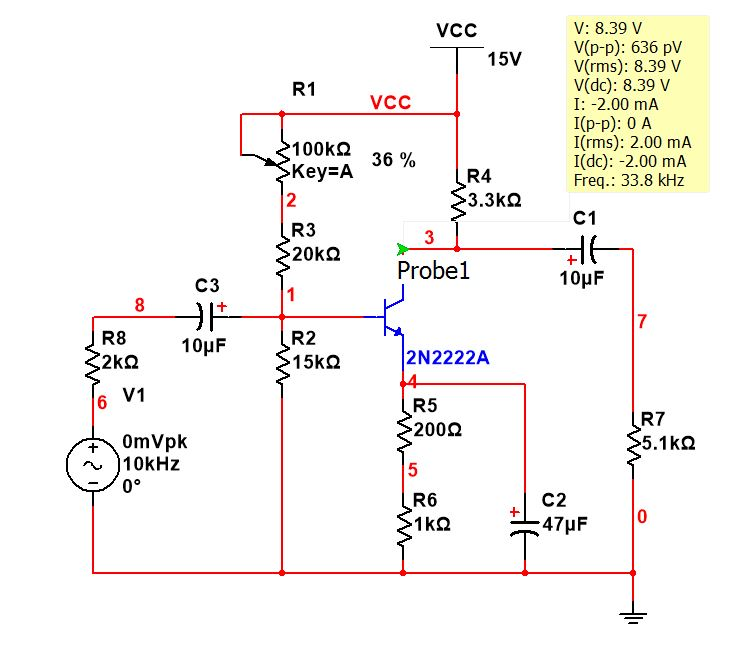
\includegraphics[width=60mm]{1-1.jpg}
\caption{单管BJT放大电路}
\label{bjtc}
\end{wrapfigure}
如图\ref{bjtc}所示是仿真采用的单管放大电路。电路采用阻容耦合方式和射级稳Q电路。经过对变阻器$R_1$的调整,使得如图所示的静态工作电流$I_c=2mA$

下面对$R_1$的数值进行理论计算。经过之前几次的仿真可以知道BJT$\beta\approx220$因此可以得到$I_c\approx I_e\approx 2\rm{mA},U_e=2.4\rm{V}$

进一步,考虑BJT的开启电源$U_{on}\approx0.7\rm{V}$因此可以得到$U_b=3.1\rm{V}$

可以认为三极管基极电流可以忽略不计,那么我们可以得到分压电阻上的电流为
$I=\frac{U_b}{R_2}=0.206\rm{mA}$并进一步得到上拉电阻阻值为$\frac{V_{cc}-U_{b}}{I}=57\mathrm{k}\Omega$

经过仿真测试,可以发现经过调整上拉电阻为$36\mathrm{k}\Omega+20\mathrm{k}\Omega=56\mathrm{k}\Omega$时系统静态工作点满足上述要求,和理论计算基本相符
\subsection{动态参数的测定}
\subsubsection{电压放大倍数的测定}
首先进行理论估算,采用三极管的中频段模型进行估算并设$r_{be}=3\mathrm{k}\Omega$可以迅速得到$A_u=-\frac{\beta(R_c//R_L)}{r_{be}}=-147$

对图\ref{bjtc}的电路外接示波器和失真度仪进行测量,可以得到如图\ref{bjtA}的波形示意图,可以得到电路的仿真放大倍数为$-frac{753+803}{5.24+5.49}=-145$发现和理论计算还是很相近的
\subsubsection{输入电阻的测定}
首先进行理论计算,根据图\ref{bjtc}电路所示,可得输入电阻$R_i=R_2//(R_1+R_3)//r_be\approx2.4\mathrm{k}\Omega$

如图\ref{bjtri}采用半压法对输入电阻进行测量,发现在输入$V_{pk}=10\rm{mV}$即$V_{rms}=7.07\rm{mV}$时,外接电阻$R_8=23.1\mathrm{k}\Omega$时可得到输入分压为3.534mV,因此可得仿真测量输入电阻为$23.1\mathrm{k}\Omega$和理论计算相差不大
\begin{figure}
\centering
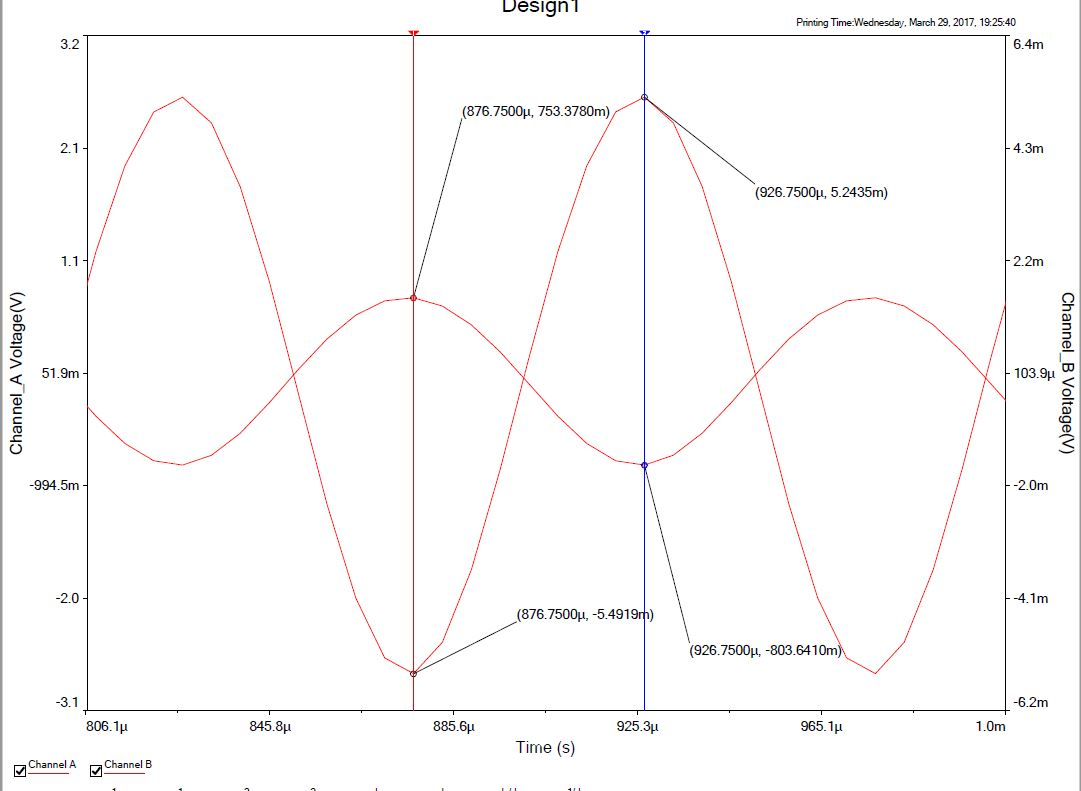
\includegraphics[width=\textwidth]{1-2AA.jpg}
\caption{电压增益的仿真波形曲线}
\label{bjtA}
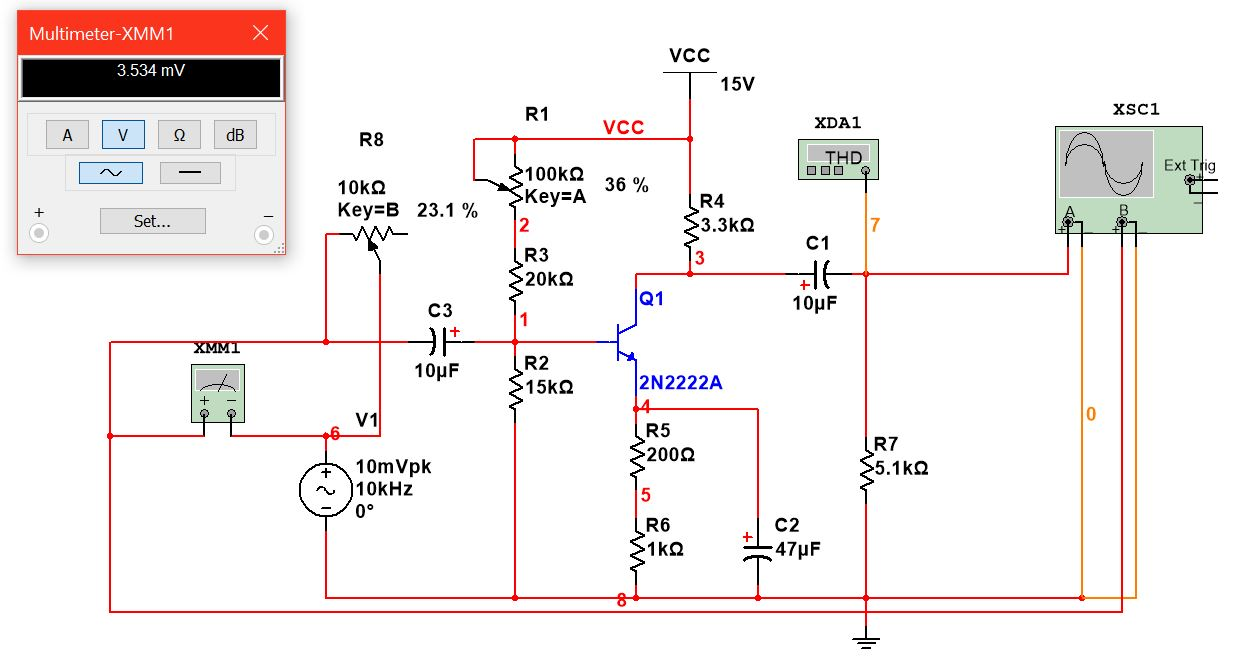
\includegraphics[width=\textwidth]{1-2Ri.jpg}
\caption{放大电路输入电阻的测量}
\label{bjtri}
\end{figure}
\subsection{输出电阻的测量}
理论计算可以迅速得到输出电阻为$3.3\mathrm{k}\Omega$

同样采取半压法进行仿真测试,首先测量空载时的输出电压有效值为888.93mV,如图\ref{bjtuo}所示,外接滑动变阻器如图\ref{bjtro},当调节至3.1$\mathrm{k}\Omega$时发现输出电压为空载输出电压的一半,因此可以得到仿真测试的输出电阻为3.1$\mathrm{k}\Omega$和理论计算值相近
\begin{figure}
\centering
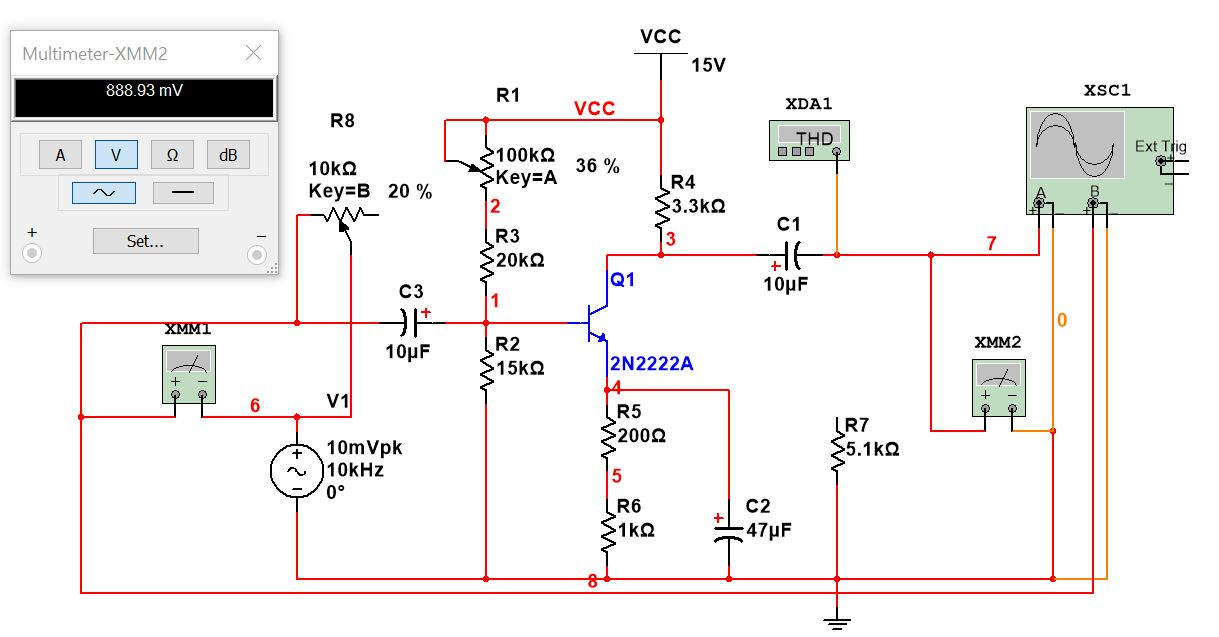
\includegraphics[width=\textwidth]{1-2Uo.jpg}
\caption{放大电路空载输出电压}
\label{bjtuo}
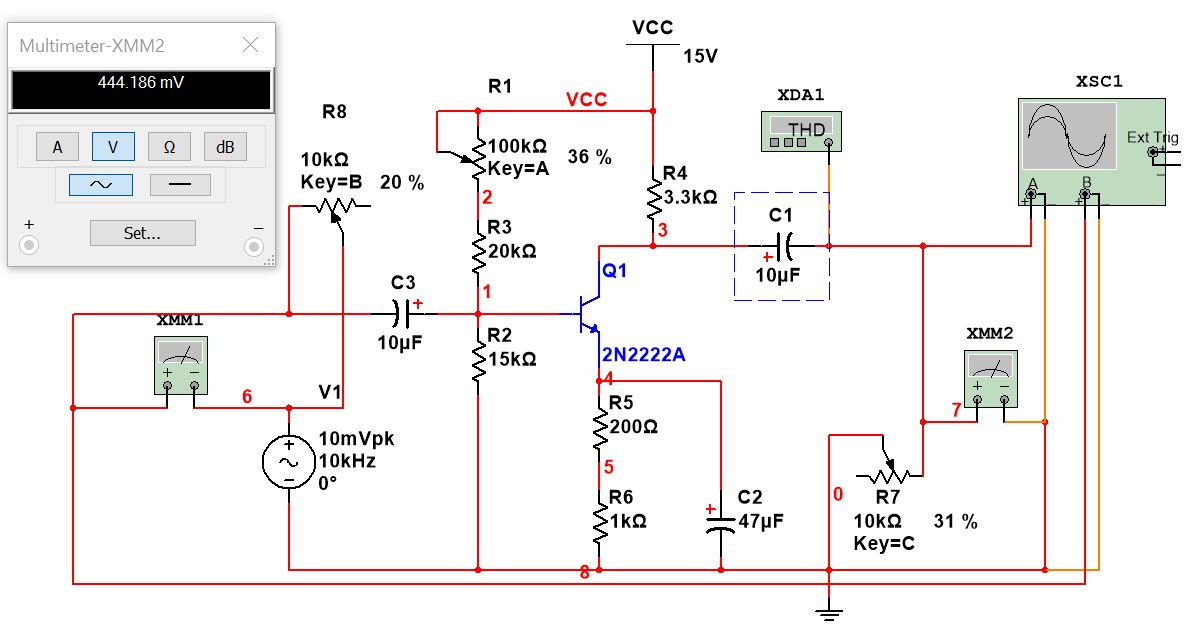
\includegraphics[width=\textwidth]{1-2Ro.jpg}
\caption{放大电路输出电阻的测量}
\label{bjtro}
\end{figure}

\subsubsection{频率响应的测试}
采用$0.707A_{us}$作为上限截止频率和下限截止频率的标准。如图\ref{bjtfl}\ref{bjtfh}所示,可得上限截止频率约为230kHz,下限截止频率为160Hz
\begin{figure}
\centering
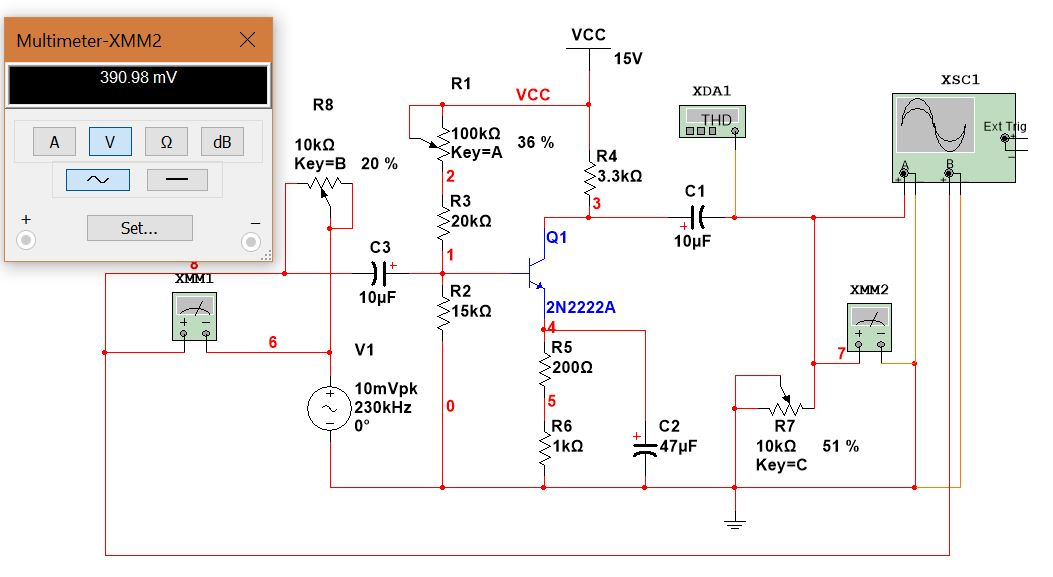
\includegraphics[width=\textwidth]{1-2fh.jpg}
\caption{上限截止频率的测试}
\label{bjtfl}
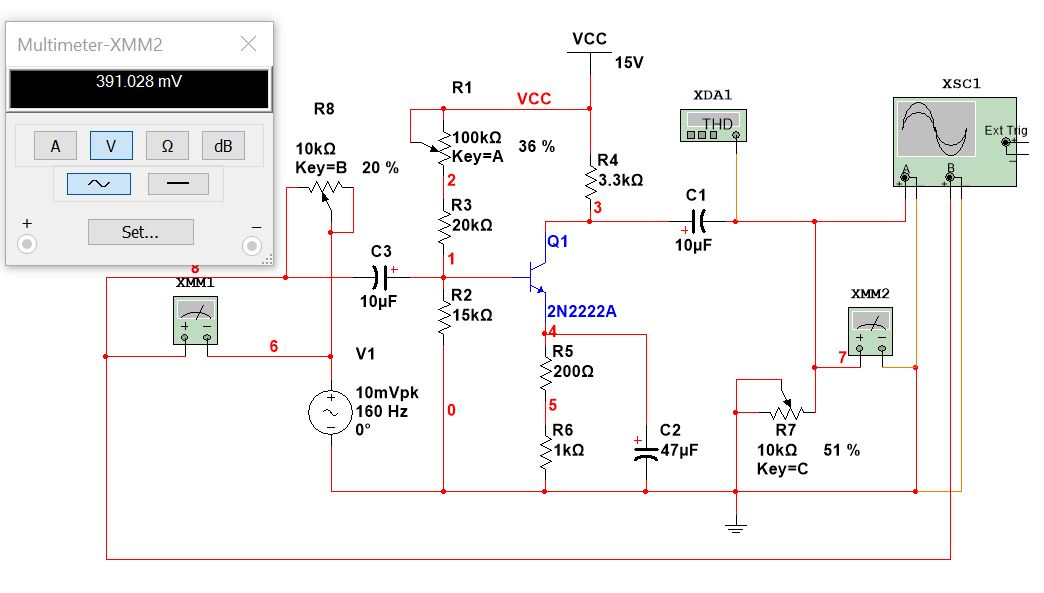
\includegraphics[width=\textwidth]{1-2fl.jpg}
\caption{下限截止频率的测试}
\label{bjtfh}
\end{figure}
\subsection{性能指标的改进}
我们希望在这个电路中能够提供较大的$A_u$,从理论上进行分析可以得到,该电路的$A_u=-\frac{\beta(R_c//R_L)}{r_{be}}$因此为实现目标我们将$R_c$从3.3$\mathrm{k}\Omega$提升至5$\mathrm{k}\Omega$,从理论上进行计算,则可得到$A_u'=-185$得到了上升

如图\ref{bjtc1}对电路进行改进,其中两个滑动变阻器的取值和图\ref{bjtc}中定值电阻的取值是相同的没有影响,可以得到如图\ref{bjtA1}的电压波形曲线,仿真测量的$A_u=-\frac{928+991}{5.16+5.45}=-180$明显得到了提升并和理论估算的值相近。同时,静态工作点没有发生变化

\begin{figure}
\centering
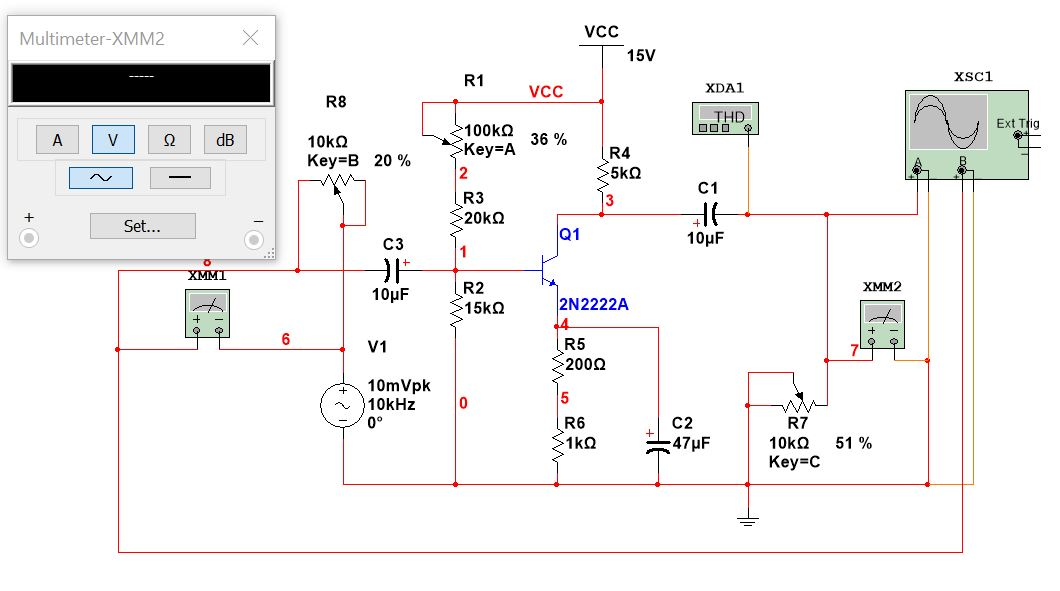
\includegraphics[width=\textwidth]{1-3Ac.jpg}
\caption{对电路的改进}
\label{bjtc1}
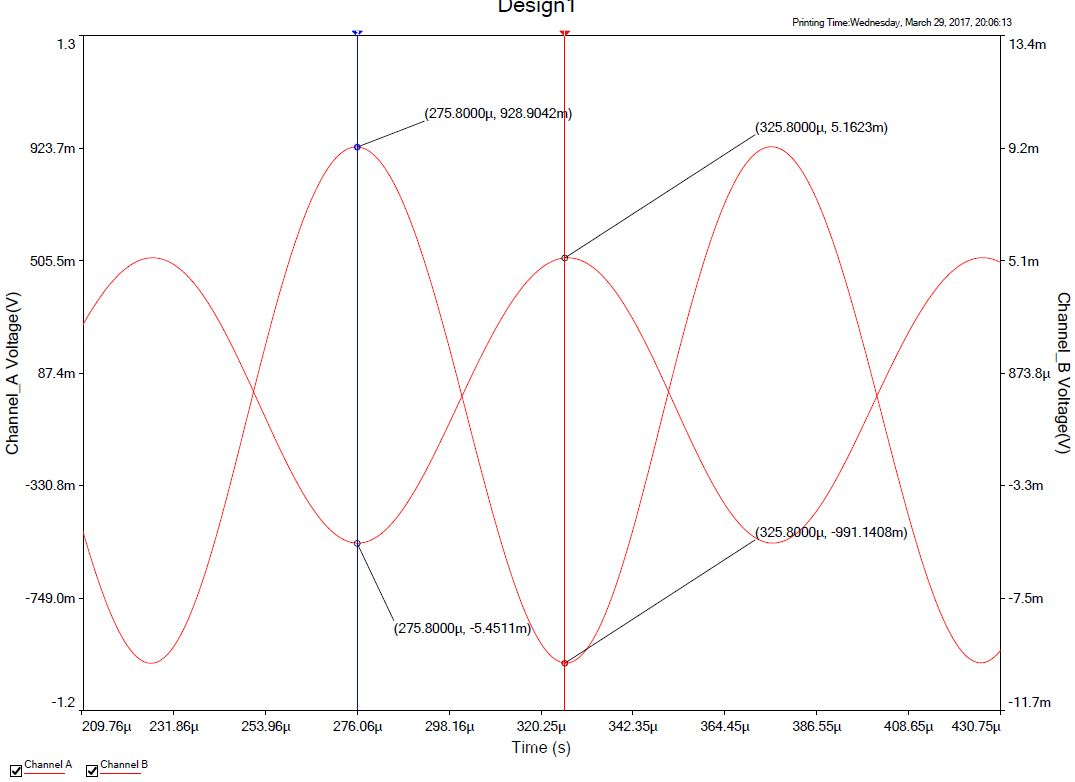
\includegraphics[width=\textwidth]{1-3AA.jpg}
\caption{改进后放大波形}
\label{bjtA1}
\end{figure}
\subsection{失真的产生和消去}
如图\ref{dist1}所示,调整$R_1$使得静态工作电流$I_c=3\rm{mA}$输入20mV信号是发生如图\ref{Adist1}所示的失真现象。显然这是底部失真,由三极管进入饱和状态引起。因此考虑提高$U_{CQ}$使三极管远离饱和状态。具体的做法是降低$R_4$。如图\ref{dist2}所示,$R_4=1\mathrm{k}\Omega$,产生的波形如图\ref{Adist2}所示,可以看出失真已经基本消除。从失真度上也可以看出明显的变化。
\begin{figure}
\centering
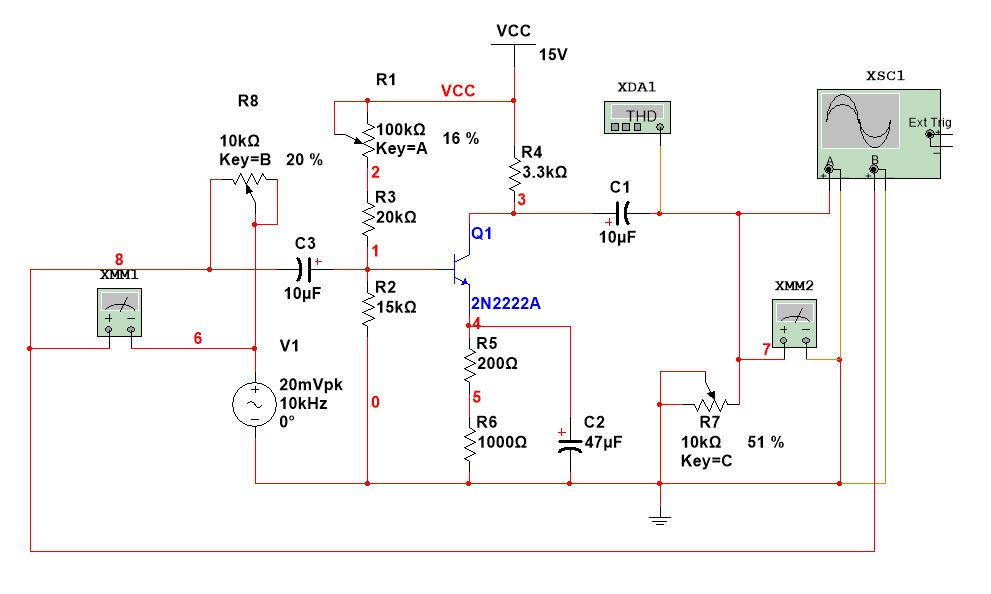
\includegraphics[width=\textwidth]{1-43mA3_3k.jpg}
\caption{失真产生电路}
\label{dist1}
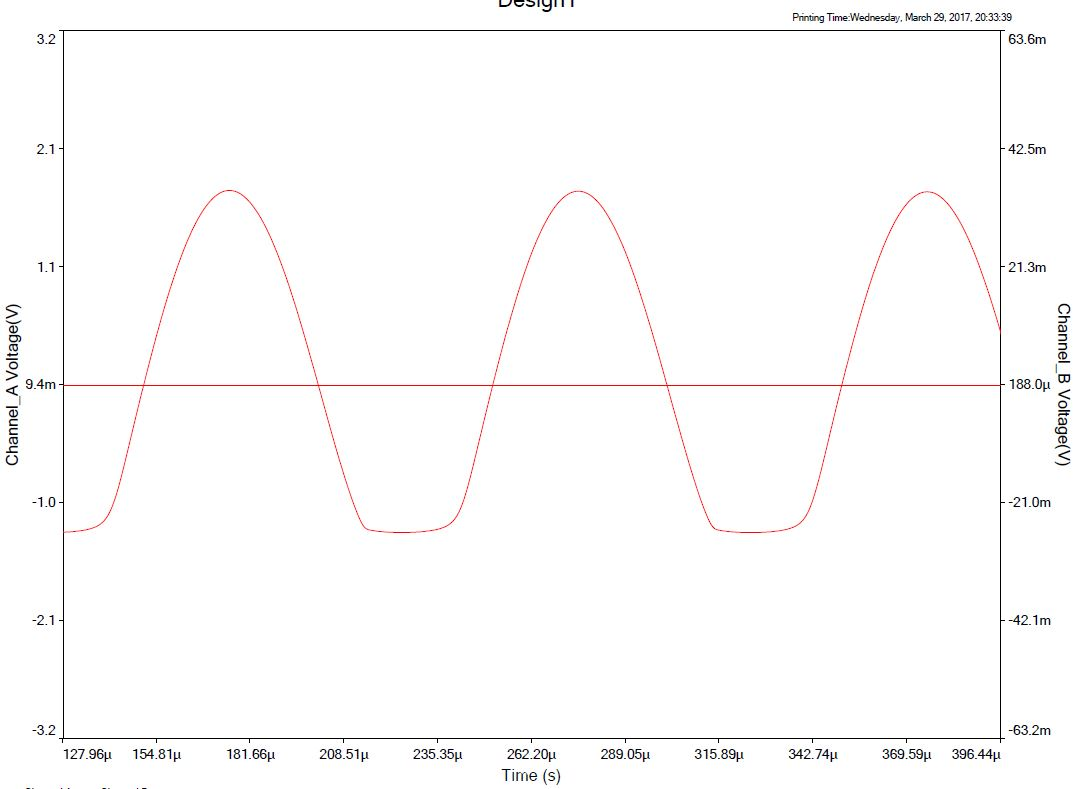
\includegraphics[width=\textwidth]{1-42.jpg}
\caption{失真波形}
\label{Adist1} 
\end{figure}

\begin{figure}
\centering
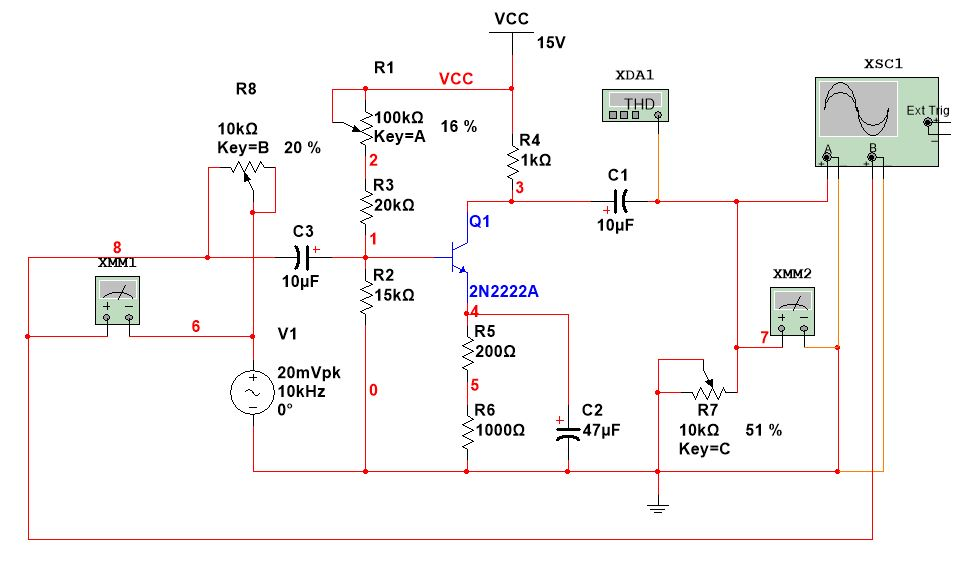
\includegraphics[width=\textwidth]{1-43mA1k.jpg}
\caption{失真消去电路}
\label{dist1}
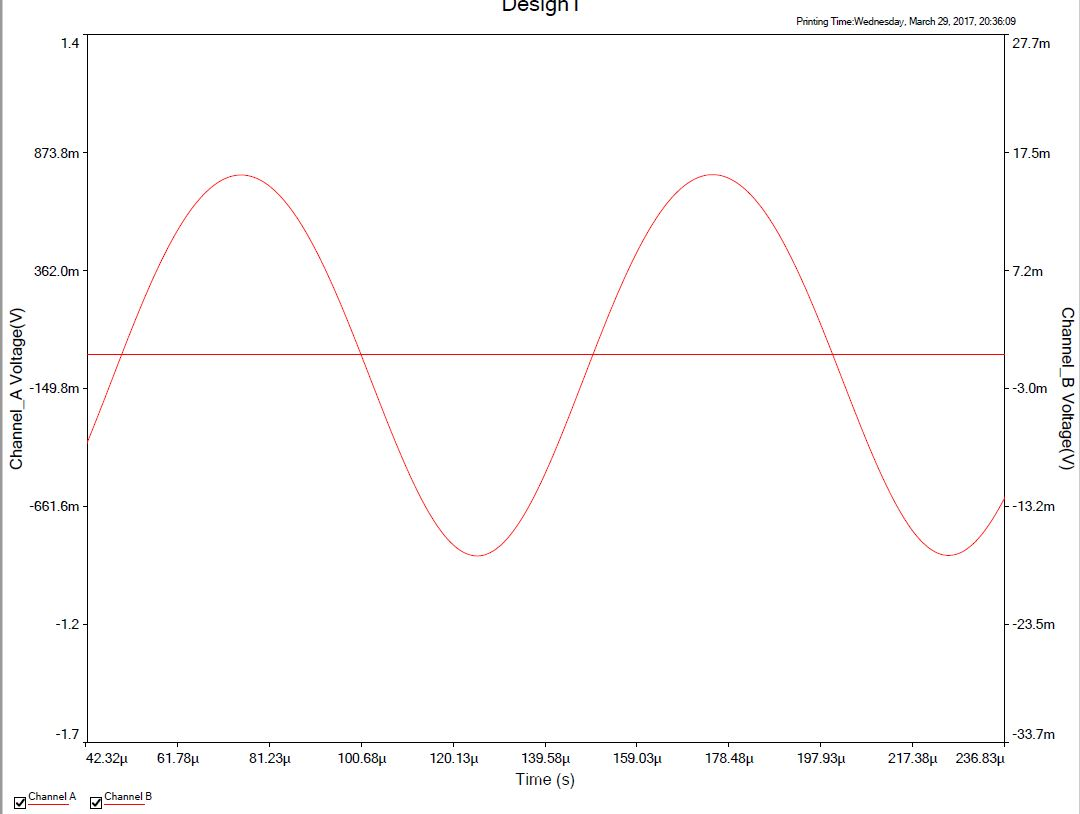
\includegraphics[width=\textwidth]{1-41.jpg}
\caption{消去失真之后的波形}
\label{Adist1} 
\end{figure}
\subsection{实际电路的搭建}
在电子技术实验课中已经完成了这方面电路的搭建,具体可见附录中的实验报告,这里就不再重复了
\clearpage
\section{单管MOS放大电路的搭建和仿真测试}
\subsection{datasheet和传输特性的测试}
\begin{wrapfigure}{r}{0pt}
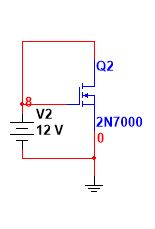
\includegraphics[width=60mm]{2-1.jpg}
\caption{2N7000输入特性测试}
\label{2in}
\end{wrapfigure}
查找相关资料可以得到NMOS管2N7000的$U_{GS(th)}$在$U_{DS}=U_{GS},I_D=250\mu\rm{A}$的测试条件下最小值为1V,最大值为3V,经典值为2.1V,按照datasheet提供的测试条件搭建如图\ref{2in}所示的测试电路,对$V_2$进行直流仿真得到如图\ref{in}的输入特性曲线,按照测试条件进行标定可得$U_{GS(th)}=2.05V$和经典值相近

下面测量MOS管在$U_{GS}=2U_{GS(th)}$时的电流$I_{D0}$,如图\ref{transfer}所示是2N7000的传输特性测试电路图,仿真时将IV测试仪选择为NMOS管测量模式,将$U_{GS}$设置为$4.1\rm{V}\approx2U_{GS(th)}$可以得到如图\ref{transfer}所示的传输特性曲线,从曲线中我们可以看出恒流区电流$I_{D0}=I_{DS}=221.2908\rm{mA}$

同时,随$U_{GS}$变化的传输特性如图\ref{whole}所示
\begin{figure}
\centering
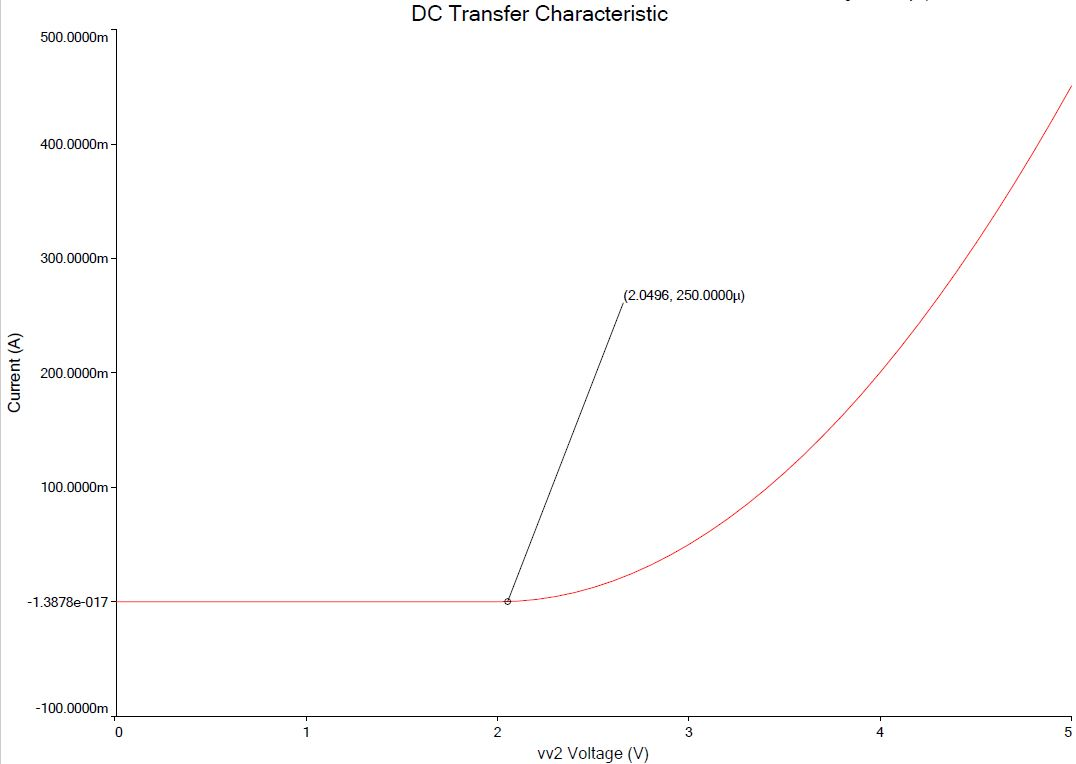
\includegraphics[width=\textwidth]{2-1in.jpg}
\caption{2N7000输入特性}
\label{in}
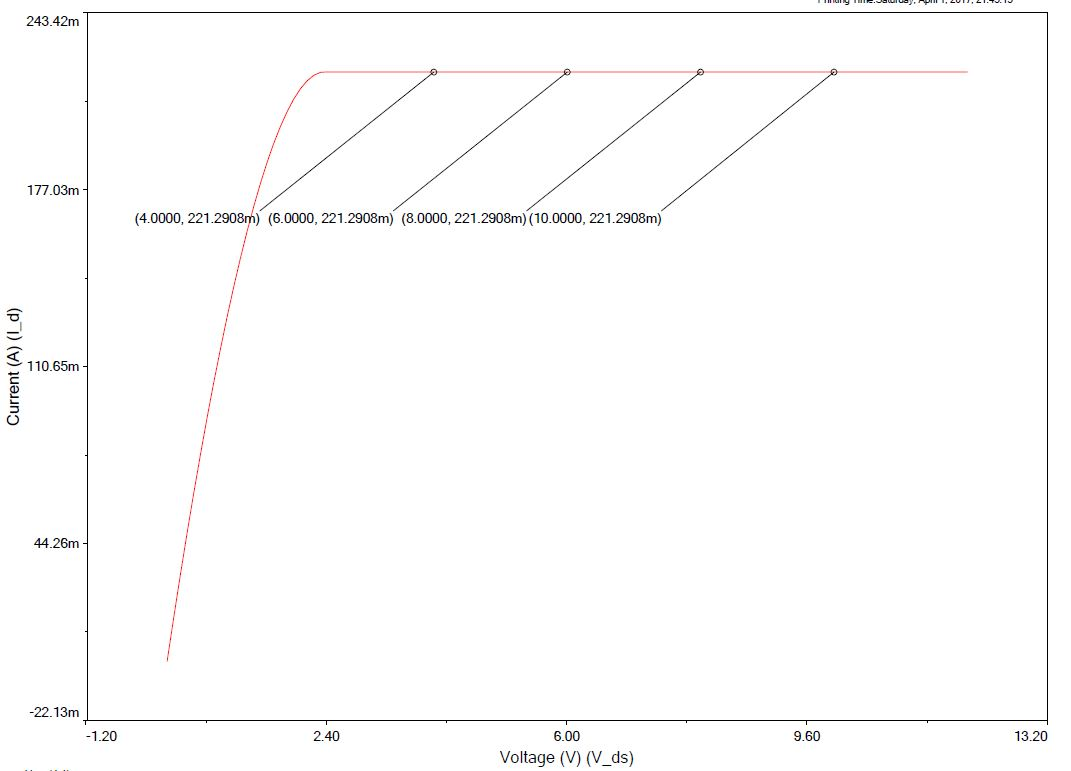
\includegraphics[width=\textwidth]{2-1out.jpg}
\caption{2N7000传输特性}
\label{transfer} 
\end{figure}
\begin{figure}
\centering
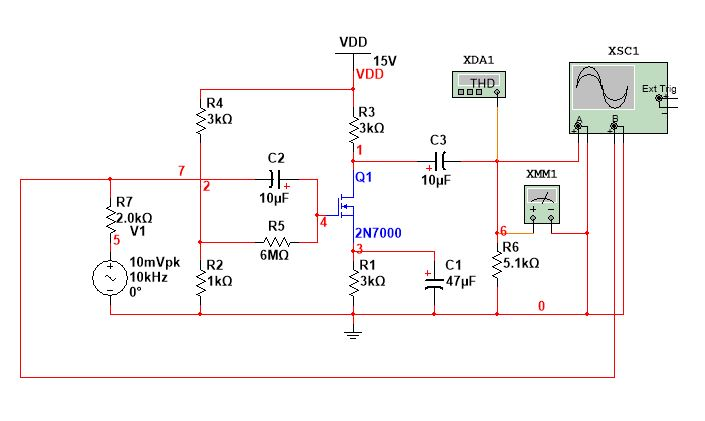
\includegraphics[width=\textwidth]{2-3.jpg}
\caption{实验电路图}
\label{MOScir}
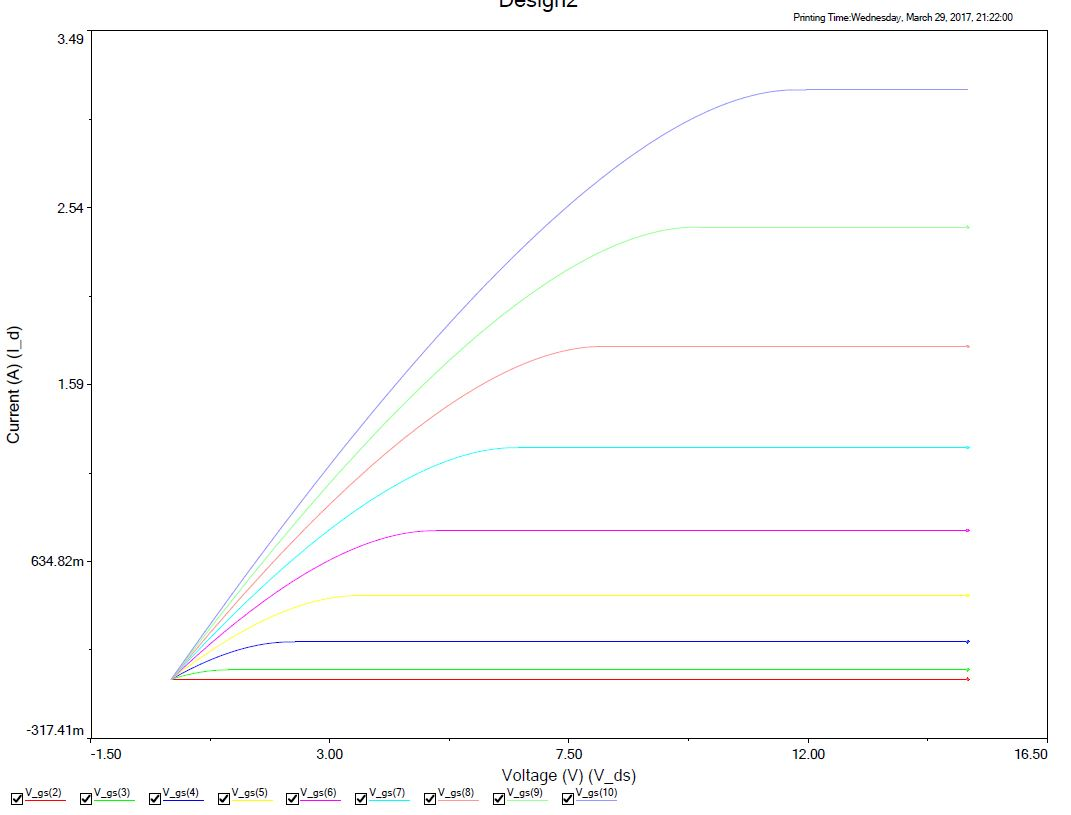
\includegraphics[width=\textwidth]{2-2.jpg}
\caption{2N7000传输特性}
\label{whole} 
\end{figure}
\subsection{静态工作点的调整}
如图\ref{MOScir}为所搭建的电路。下面进行对静态工作点的理论分析

从NMOS管的特性方程可以得到$I_{DSQ}=\frac{I_{D0}}{U_{GS(th)}^2}(3.75-I_{DSQ}R_1-U_{GS(th)})^2$解得$I_{DSQ}=0.6\rm{mA}$
并且有$U_G=3.75\rm{V},U_S=1.8\rm{V},U_D=13.19\rm{V}$

仿真电路测得实际静态工作电流为589$\mu\rm{A}$和理论计算值相近,同时测得$U_G=3.75\rm{V},U_S=1.65\rm{V},U_D=13.4\rm{V}$
均和理论计算相差不大。测试电路图采用探针进行测量,为节省篇幅这里略去。
\subsection{动态参数的测定}
\subsubsection{电压放大倍数的测定}
首先进行理论估算,可以计算得到MOS管的$g_m=2\sqrt{I_{D0}I_{DSQ}}/U_{GS(th)}=11.13\rm{mA/V}$同时进一步得到电压放大倍数为$A_u=-g_m(R3//R_L)=-21$

对图\ref{MOScir}的电路外接示波器和失真度仪进行测量,可以得到如图\ref{MOSA}的波形示意图,可以得到电路的仿真放大倍数为$-frac{189+207}{20}=-19.8$发现和理论计算还是很相近的
\subsubsection{输入电阻的测定}
首先进行理论计算,根据图\ref{MOScir}电路所示,可得输入电阻$R_i=\approx6\mathrm{M}\Omega$

如图\ref{MOSri}采用半压法对输入电阻进行测量,发现在输入$V_{pk}=10\rm{mV}$即$V_{rms}=7.07\rm{mV}$时,外接电阻$R_8=78\mathrm{k}\Omega$时可得到输入分压为3.534mV,因此可得仿真测量输入电阻为$78\mathrm{k}\Omega$和理论计算有很大差异,后采用探针法进行测量,发现在$V_{pp}=20\rm{mV}$时,$I_{pp}=150\rm{nA}$输入电阻仍在$100\mathrm{k}\Omega$的数量级,考虑可能因为2N7000GS之间的漏电电流导致的小输入电阻。可以通过在输入端口并联分流电阻解决问题
\begin{figure}
\centering
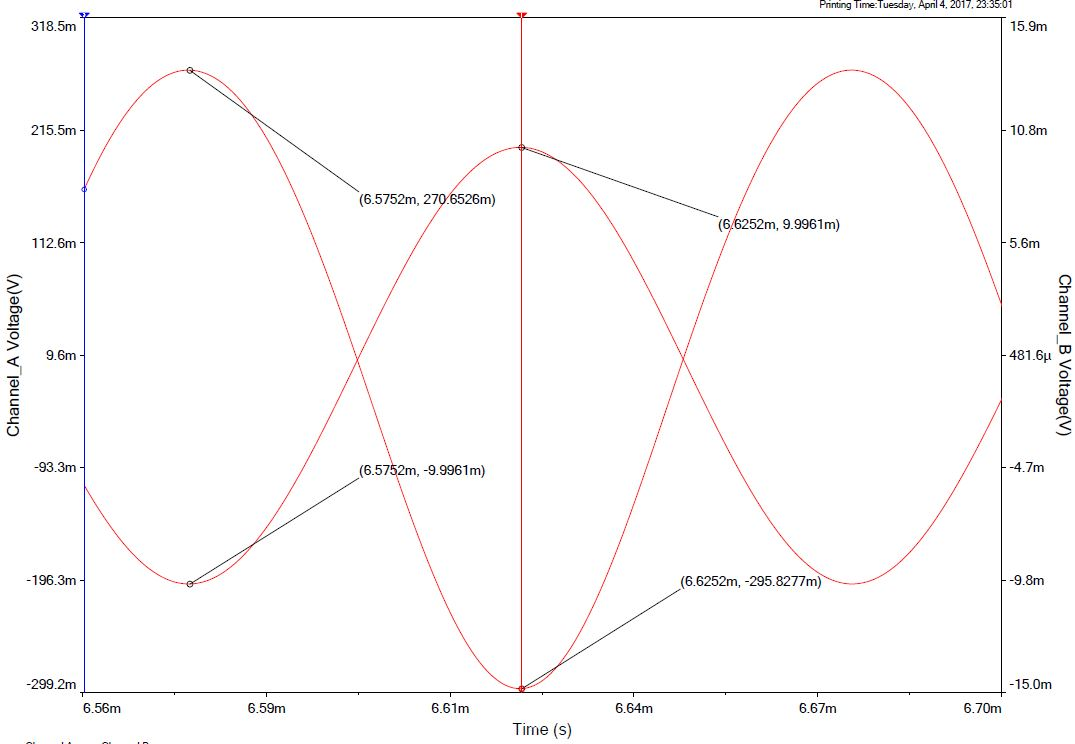
\includegraphics[width=\textwidth]{2-3AA.jpg}
\caption{电压增益的仿真波形曲线}
\label{MOSA}
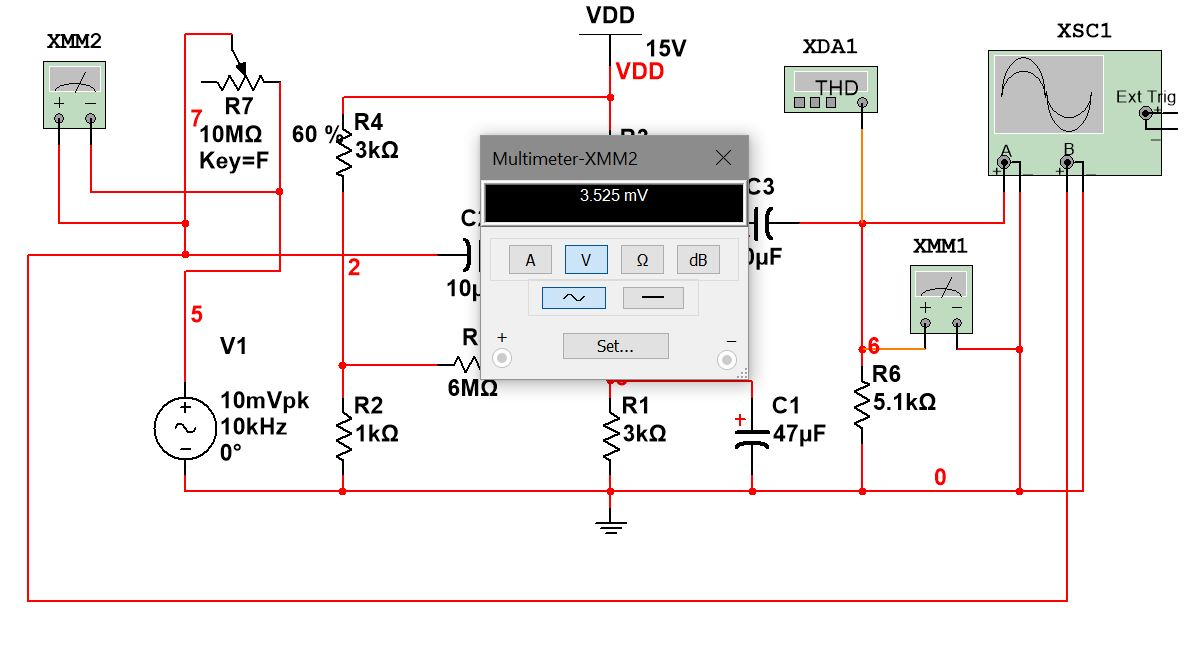
\includegraphics[width=\textwidth]{2-4Ri.jpg}
\caption{放大电路输入电阻的测量}
\label{MOSri}
\end{figure}
\subsection{输出电阻的测量}
理论计算可以迅速得到输出电阻为$3\mathrm{k}\Omega$

同样采取半压法进行仿真测试,首先测量空载时的输出电压有效值为222mV,外接滑动变阻器如图\ref{MOSro},当调节至3$\mathrm{k}\Omega$时发现输出电压为空载输出电压的一半,因此可以得到仿真测试的输出电阻为3$mathrm{k}\Omega$和理论计算值相近
\begin{figure}
\centering
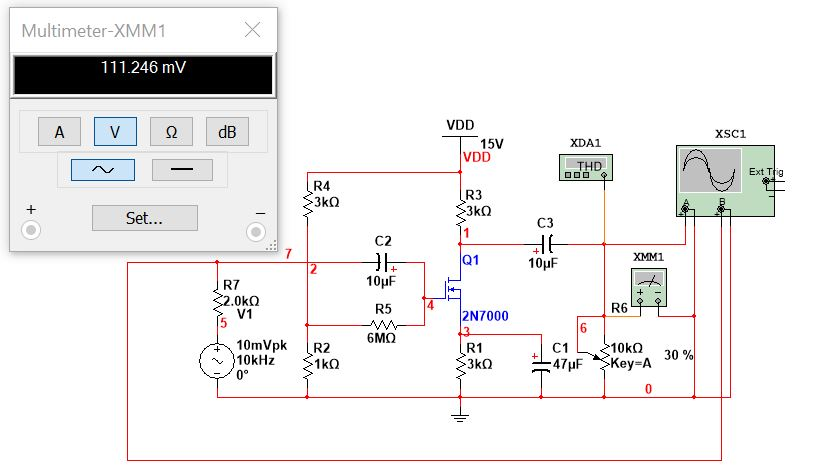
\includegraphics[width=\textwidth]{2-4Ro.jpg}
\caption{放大电路输出电阻的测量}
\label{MOSro}
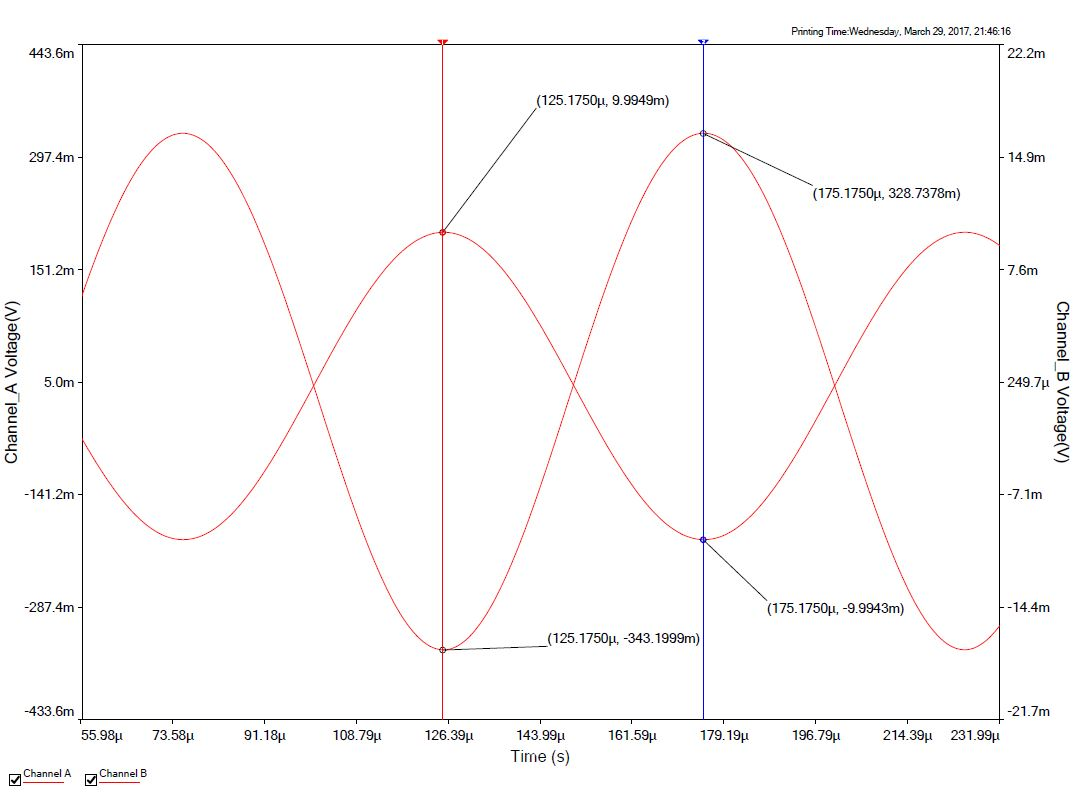
\includegraphics[width=\textwidth]{2-4AA.jpg}
\caption{改进的输出电压放大倍数}
\label{AAA}
\end{figure}

\subsubsection{频率响应的测试}
采用$0.707A_{us}$作为上限截止频率和下限截止频率的标准。如图\ref{MOSfl}\ref{MOSfh}所示,可得上限截止频率约为435kHz,下限截止频率为40Hz
\begin{figure}
\centering
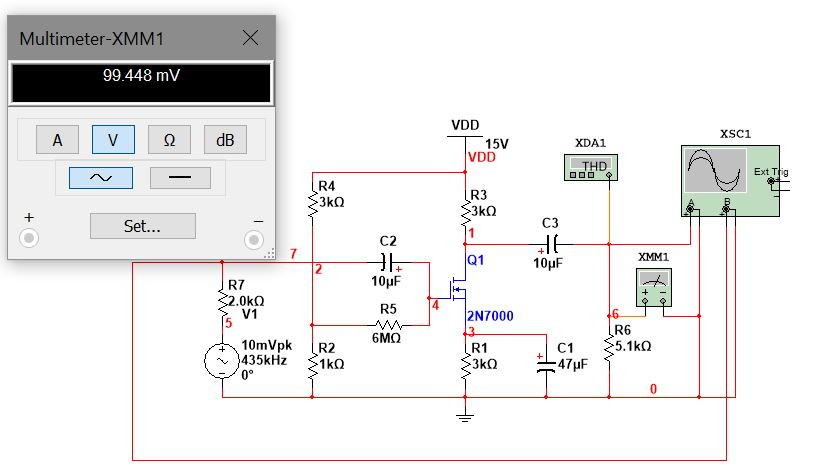
\includegraphics[width=\textwidth]{2-4fh.jpg}
\caption{上限截止频率的测试}
\label{MOSfl}
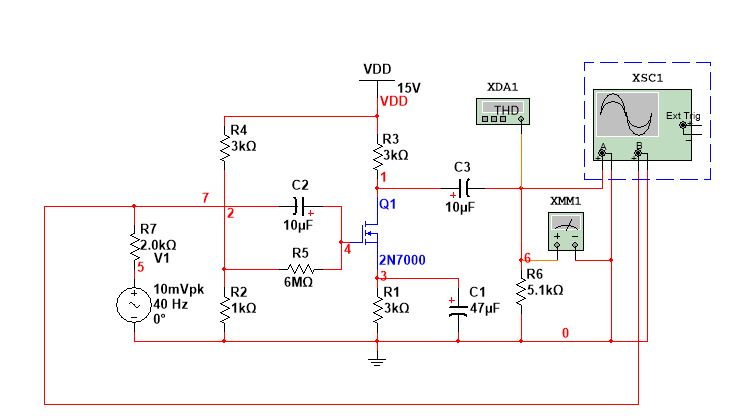
\includegraphics[width=\textwidth]{2-4fl.jpg}
\caption{下限截止频率的测试}
\label{MOSfh}
\end{figure}
\subsection{性能指标的改进}
希望提高电压放大倍数A,考虑到$A_u=-g_m(R3//R_L)$因此可以通过增大$R_3$来提高电压放大倍数,令$R_3=8\mathrm{k}\Omega$得到对应的电压放大倍数理论值为-34.66从理论上看的确得到了提升

实际仿真如图\ref{AAA}所示,可以测得电压放大倍数为$-\frac{343+328}{20}=-33.55$可以发现电压放大倍数的确得到了提升
\subsection{失真的产生和消去}
将输入电压峰峰值调整至50mV,如图\ref{WG}所示可以明显看出出现了失真,这是顶部失真,由于MOS管进入截止区产生,因此想要消除这种失真,必须提升$U_{GS}$,因此采用将下拉电阻增大即$R_2=3\mathrm{k}\Omega$,仿真波形如\ref{FG}所示发现失真得到明显的消去

\begin{figure}
\centering
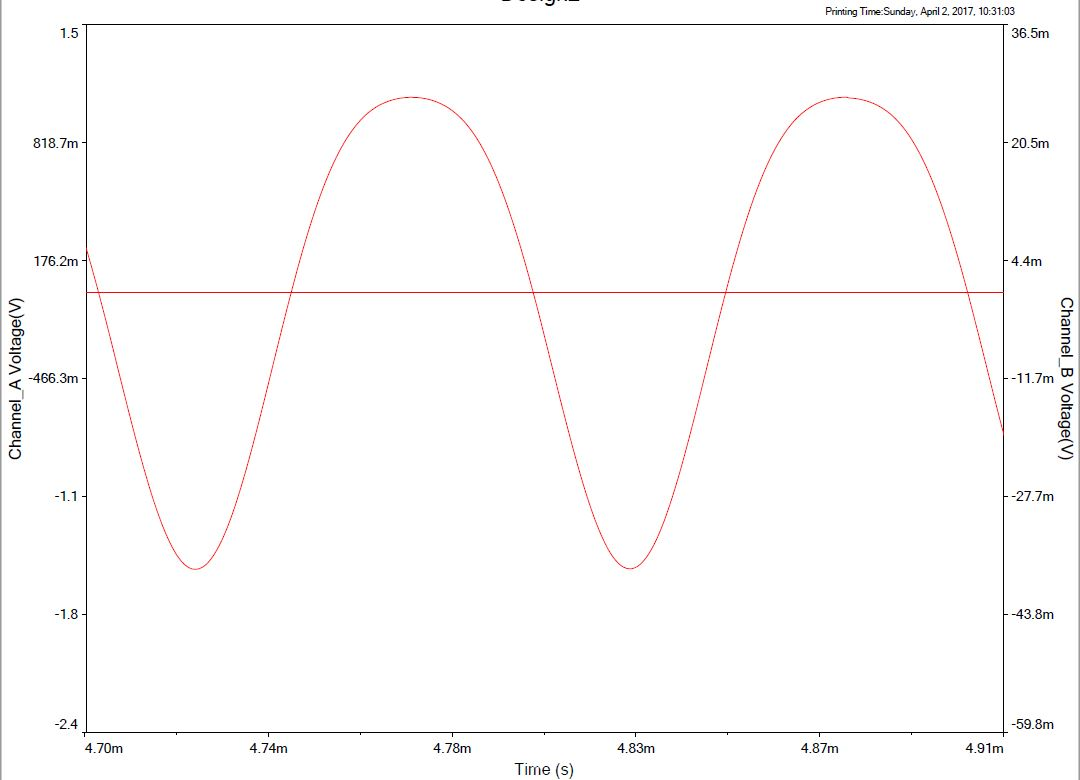
\includegraphics[width=\textwidth]{2-5W.jpg}
\caption{失真的产生}
\label{WG}
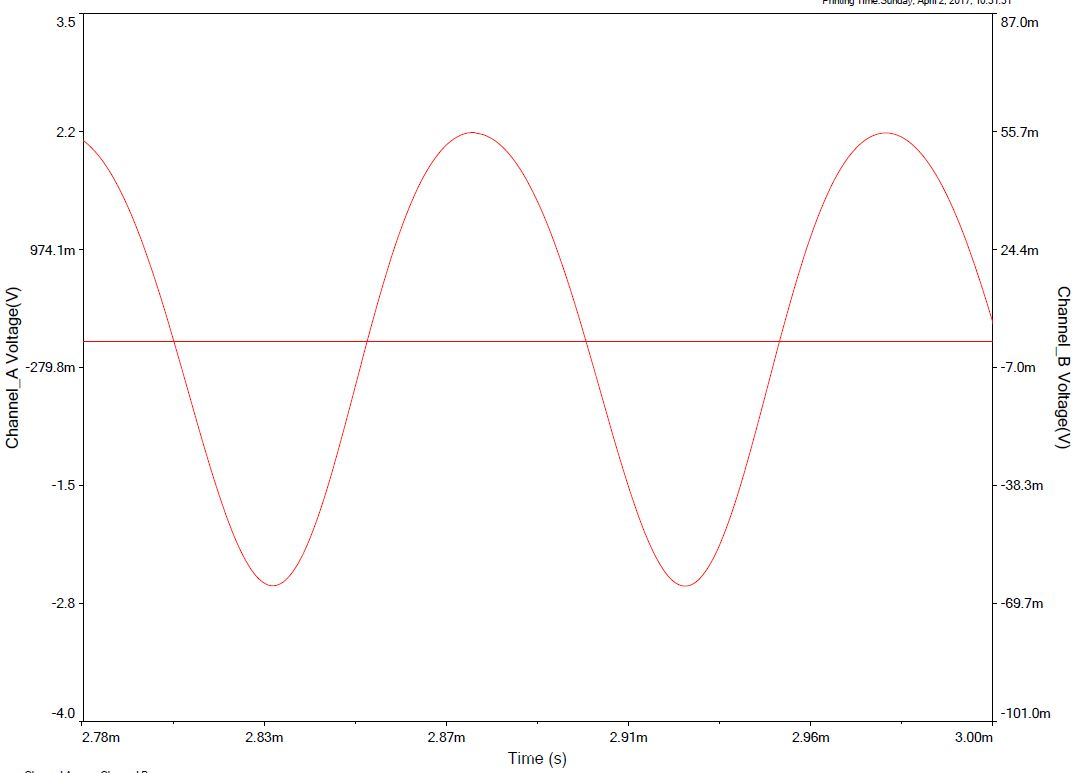
\includegraphics[width=\textwidth]{2-5F.jpg}
\caption{失真的消去}
\label{FG}
\end{figure}
\subsection{实际电路的搭建}
因为时间有限,此选做任务没有完成
\clearpage
\section{集成运放的搭建和仿真测试}
\subsection{电路的搭建}
如图\ref{CCCC}所示,参考F007型集成运放的电路设计,完成了电路的搭建,同时调整电阻$R_5=21.15\mathrm{k}\Omega,C=0\rm{pF}$对电路的低频特性进行了调整,同时保证电路输入端没有电压时输出端电压尽可能接近0V
\subsection{静态工作点的确定}
经过调整,电路的静态工作点如图\ref{static}所示,因为静态工作参数太多这里就不逐一叙述了
\begin{figure}
\centering
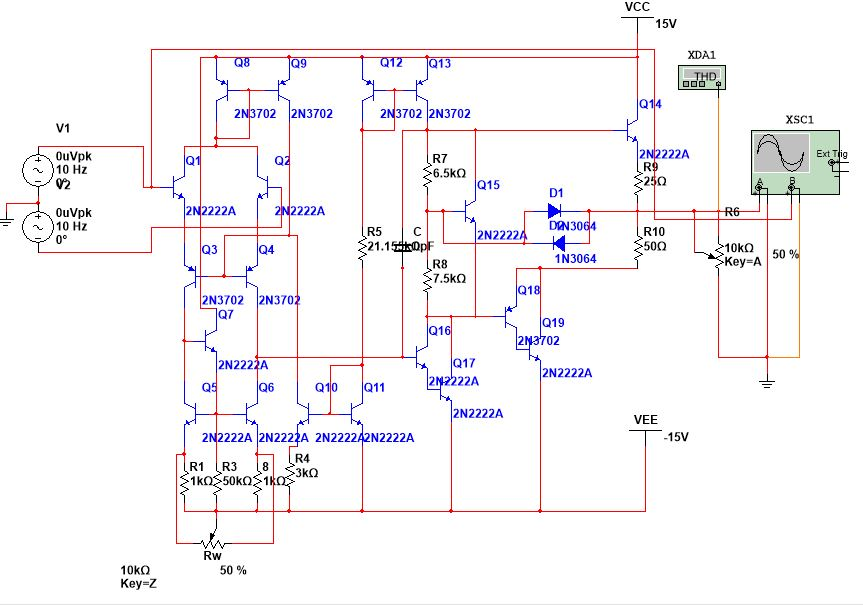
\includegraphics[width=\textwidth]{3c.jpg}
\caption{集成运放工作电路}
\label{CCCC}
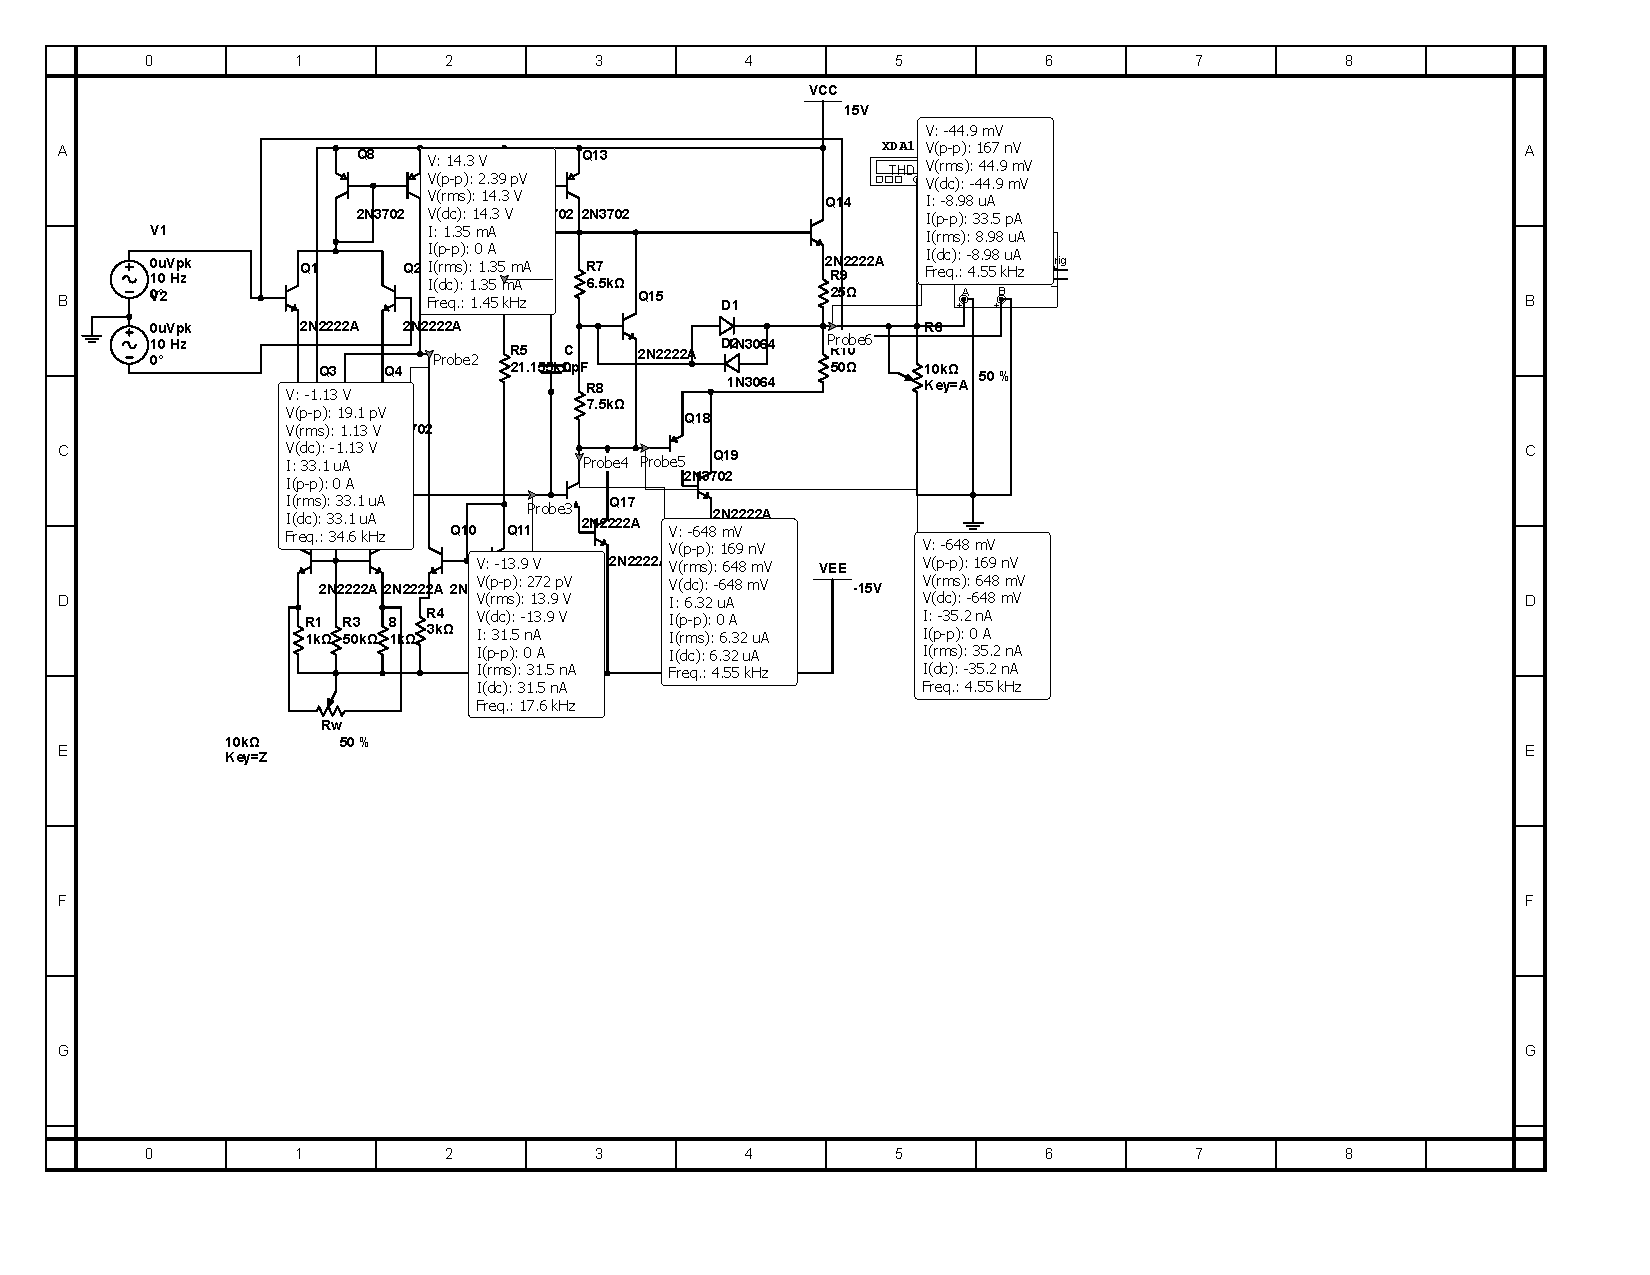
\includegraphics[width=\textwidth]{3-3static.jpg}
\caption{集成运放静态工作点}
\label{static}
\end{figure}
\subsection{动态参数的测定}
\subsubsection{电压放大倍数的测定}
如图\ref{AC}所示测量电压放大倍数,其中原信号由中间抽头接地测量,因此电压实际上为原来的2倍,可以计算得到电压放大倍数为$-\frac{300m+298.6m}{2u}=-3\times10^5$在集成运放信号放大的数量级内
\begin{figure}
\centering
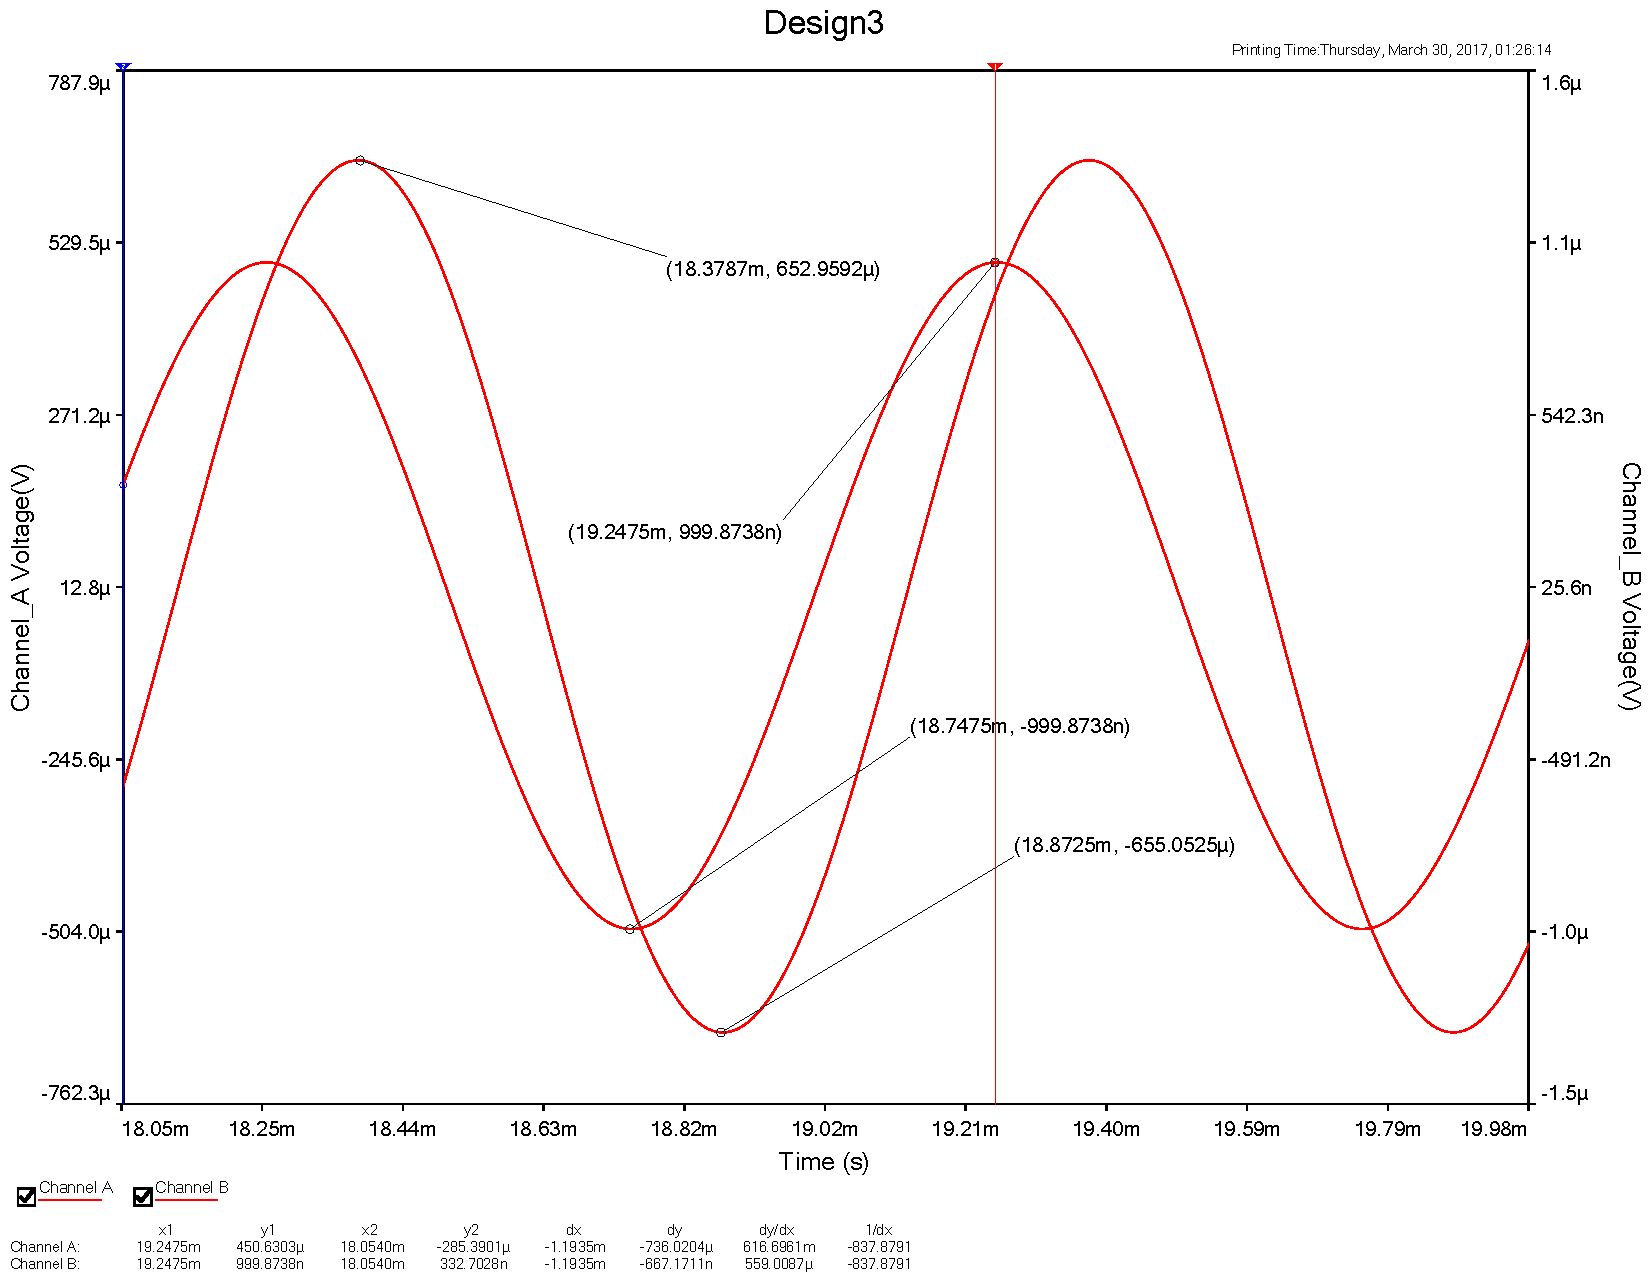
\includegraphics[width=\textwidth]{3-3A.jpg}
\caption{集成运放放大倍数}
\label{AC}
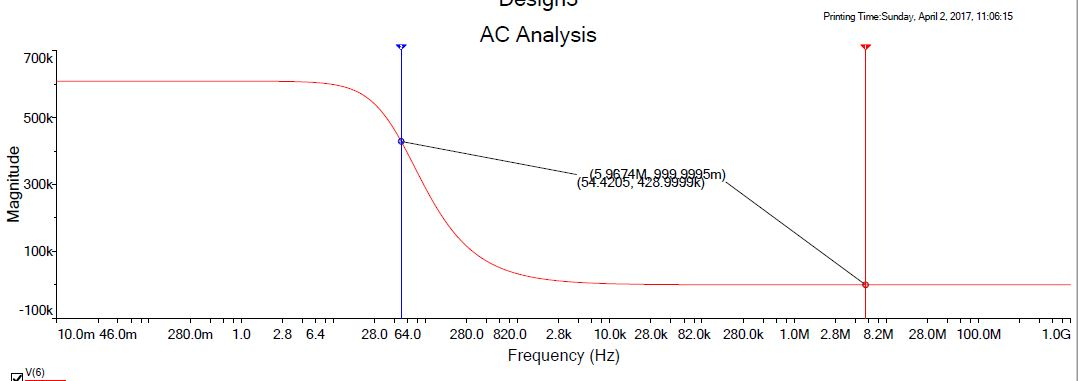
\includegraphics[width=\textwidth]{3f.JPG}
\caption{集成运放频率特性}
\label{f}
\end{figure}
\subsubsection{输入电阻的测量}
如图\ref{CRi}测量输入电阻,因为电路输入电阻很大,因此直接采用探针进行测量,如图\ref{BRI}所示,测得输入电流可以估计为$45\rm{fA}$,输入电压为$1\mu\rm{V}$

因此可以得到输入电阻为$22\mathrm{M}\Omega$基本符合集成运放的工作特性
\begin{figure}
\centering
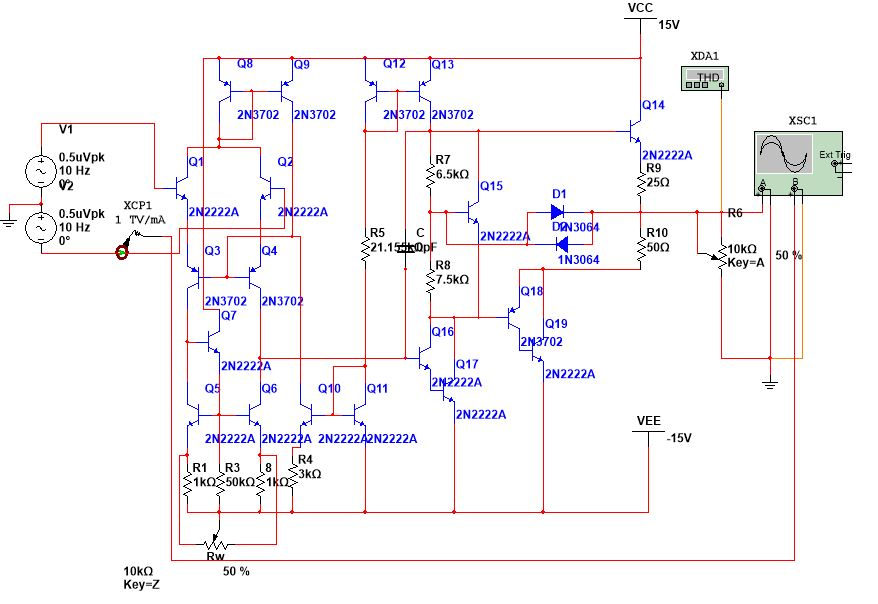
\includegraphics[width=\textwidth]{3-4Ri.jpg}
\caption{输入电阻测量电路}
\label{CRi}
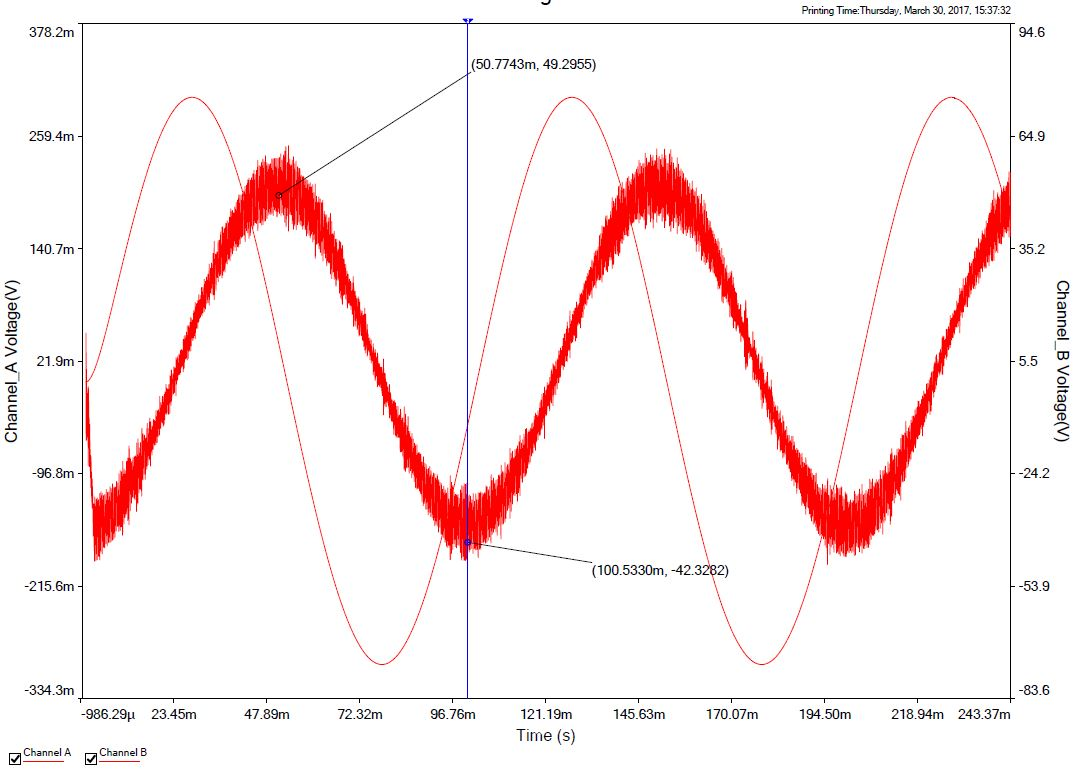
\includegraphics[width=\textwidth]{3-4Rbi.jpg}
\caption{输入电流}
\label{BRI}
\end{figure}
\subsubsection{输出电阻的测定}
采取半压法进行仿真测试,首先测量空载时的输出电压峰值为300mV,如图\ref{uo}所示,外接滑动变阻器如图\ref{ro},当调节至$100\Omega$时发现输出电压为空载输出电压的一半,因此可以得到仿真测试的输出电阻为$100\Omega$
\begin{figure}
\centering
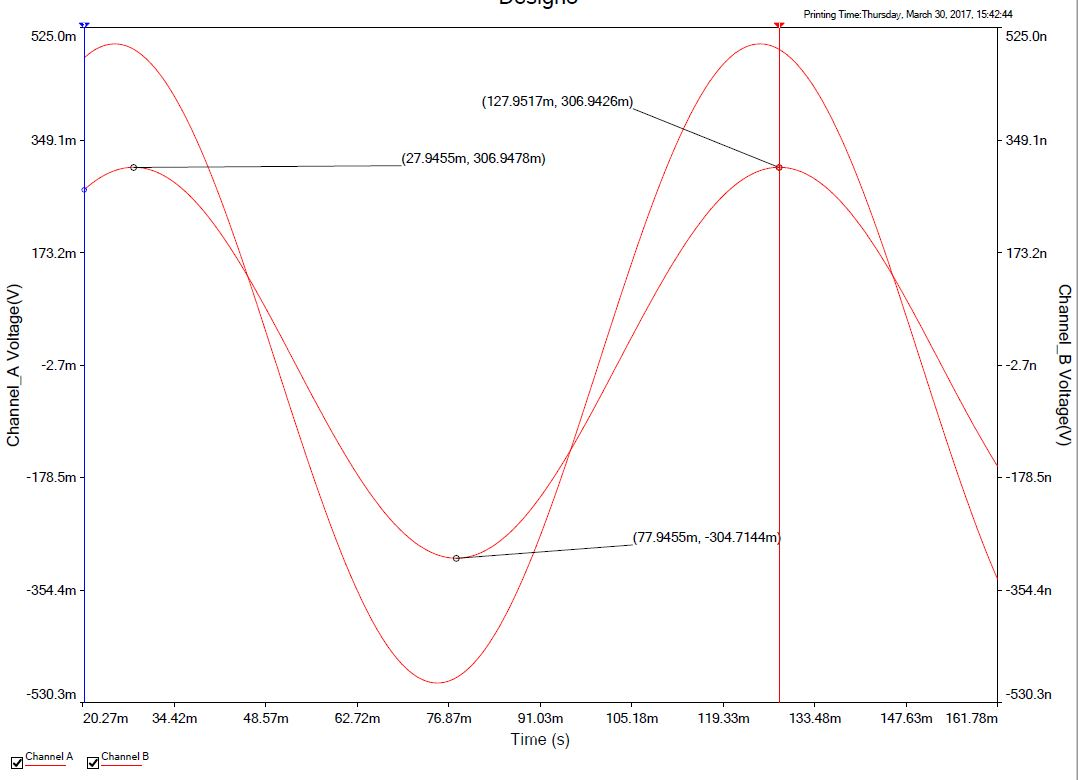
\includegraphics[width=\textwidth]{3-4Uo.jpg}
\caption{集成运放电路空载输出电压}
\label{uo}
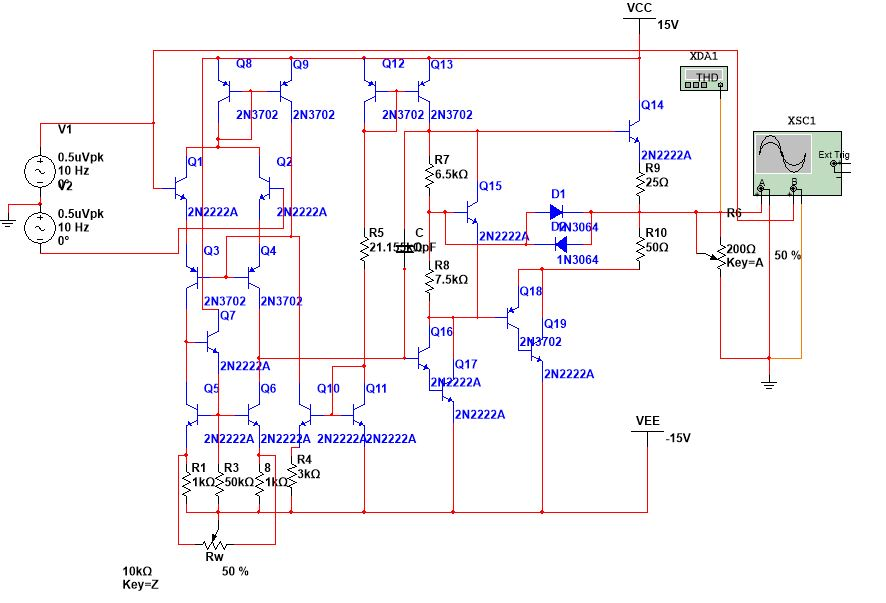
\includegraphics[width=\textwidth]{3-4Ro.jpg}
\caption{集成运放输出电阻的测量}
\label{ro}
\end{figure}
\subsubsection{频率特性的测量}
如图\ref{f}所示是集成运放的频率响应,读图立刻可知$f_{bw}=54\rm{Hz},f_C=5.96\rm{MHz}$
\subsubsection{$U_{IO},I_{IO},I_{IB}$的测量}
将电路中的输入电压置零,可得$U_O=30\rm{mV}$因此可以得到$U_{IO}=\frac{30m}{3\times10^5}=1\times10^{-8}$,因为仿真中专门为优化$U_{IO}$调整了电路参数,因此$U_{IO}$性能很好

简单测量可以得到$I_{IO}=2.6\rm{nA},I_{IO}=1.21\mu\rm{A}$
\subsubsection{SR特性的测试}
如图\ref{CSR}所示将输入电压源换位等值的方波,测量波形如图\ref{SR}所示。按照95\%定义的恢复时间计算,可得$SR=\frac{1.4723}{908.85m}=1.61\rm{V/S}$
\begin{figure}
\centering
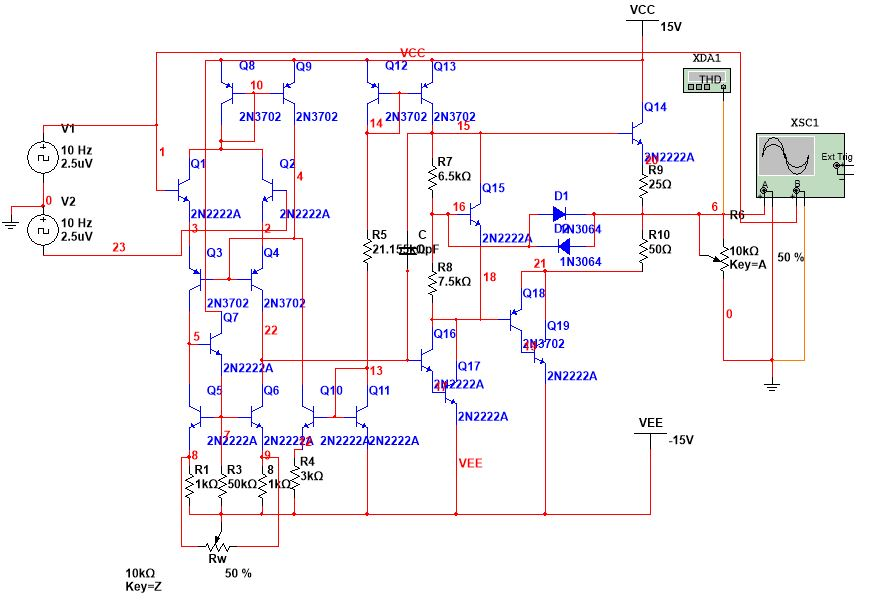
\includegraphics[width=\textwidth]{CSR.jpg}
\caption{集成运放SR特性测试电路}
\label{CSR}
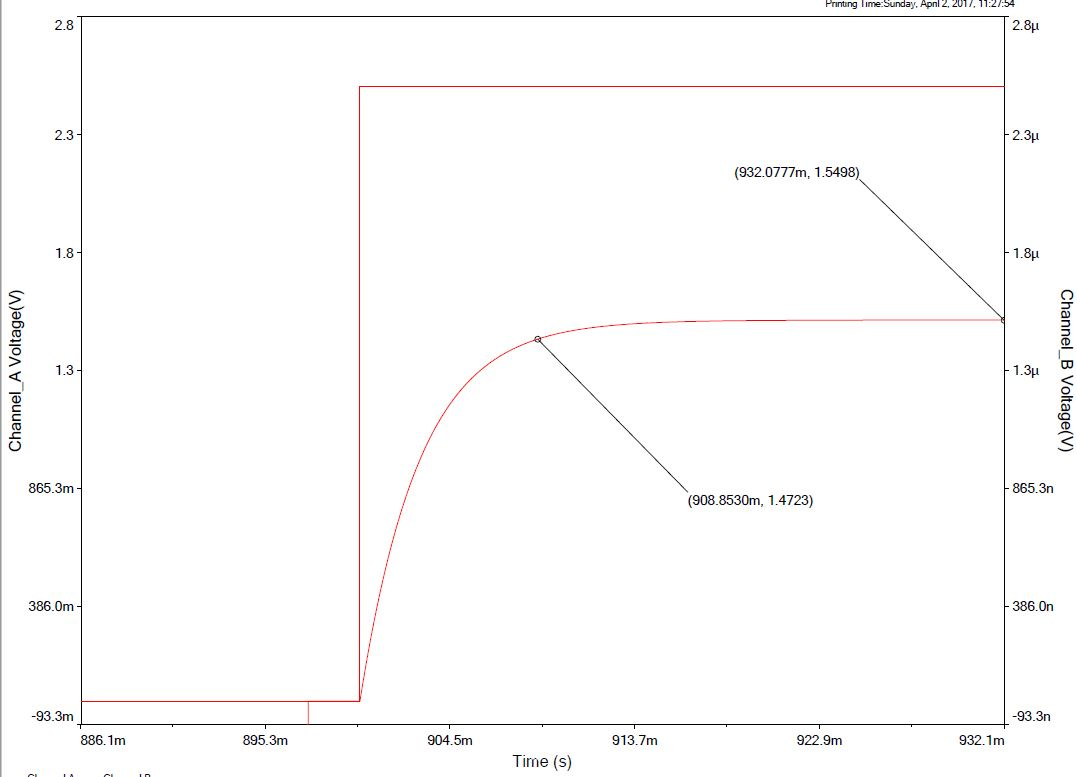
\includegraphics[width=\textwidth]{SR.jpg}
\caption{集成运放SR特性}
\label{SR}
\end{figure}
\section{负反馈放大电路自激震荡的产生和消去}
\subsection{自激震荡的产生}
从图\ref{f}中可以看出3中搭建的运放是一个闭环稳定的系统,不能产生自激震荡,因此考虑在输出端并联一个电容降低稳定性,如图\ref{c1}所示,得到电路如图\ref{CC}所示,bode图如\ref{boode}所示,可以看出系统不论是相角裕度还是幅值裕度均不满足闭环稳定条件,系统闭环不稳定。仿真出现如图\ref{exp}的自激震荡,幅值大约为20mV,已经影响正常工作
\begin{figure}
\centering
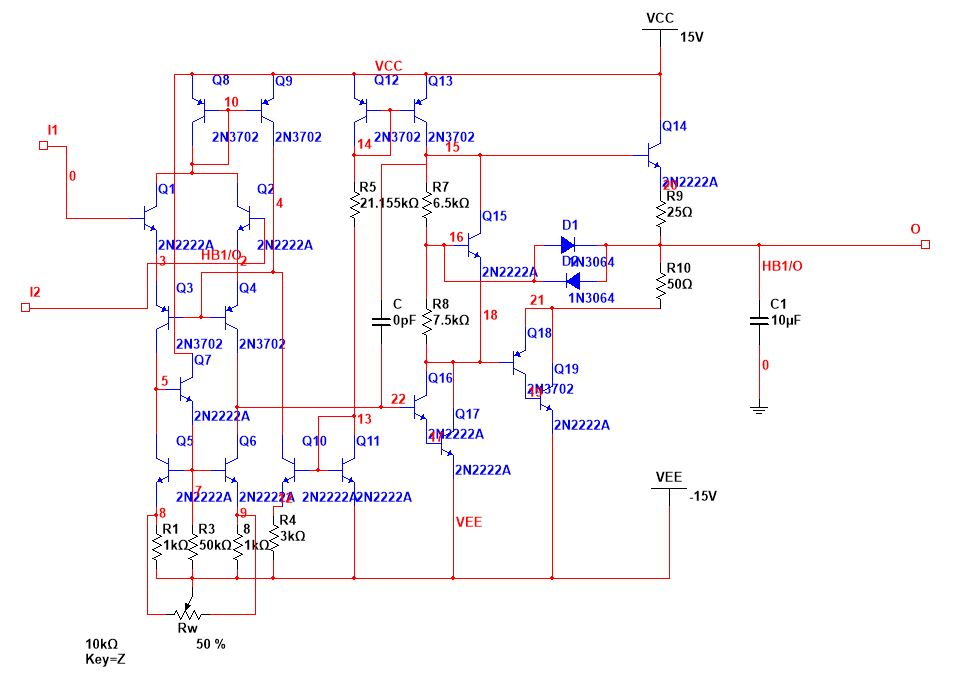
\includegraphics[width=\textwidth]{4-c2.jpg}
\caption{集成运放的封装和调整}
\label{c1}
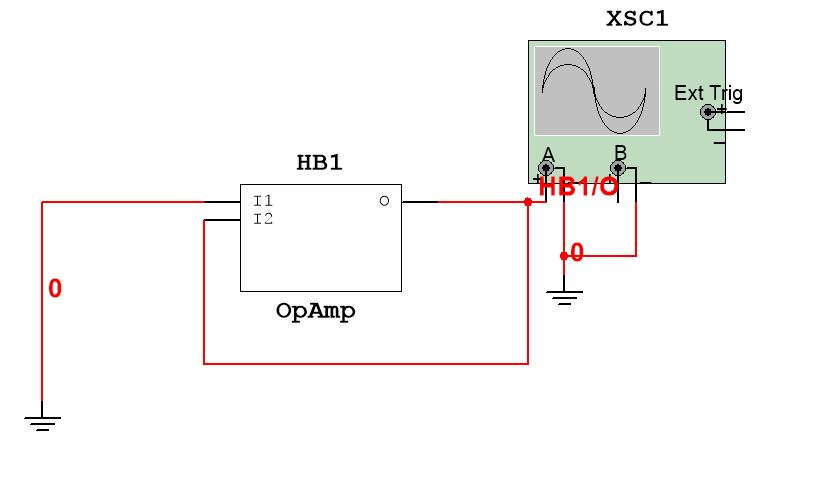
\includegraphics[width=\textwidth]{4-c.jpg}
\caption{外部电路图}
\label{CC}
\end{figure}
\begin{figure}
\centering
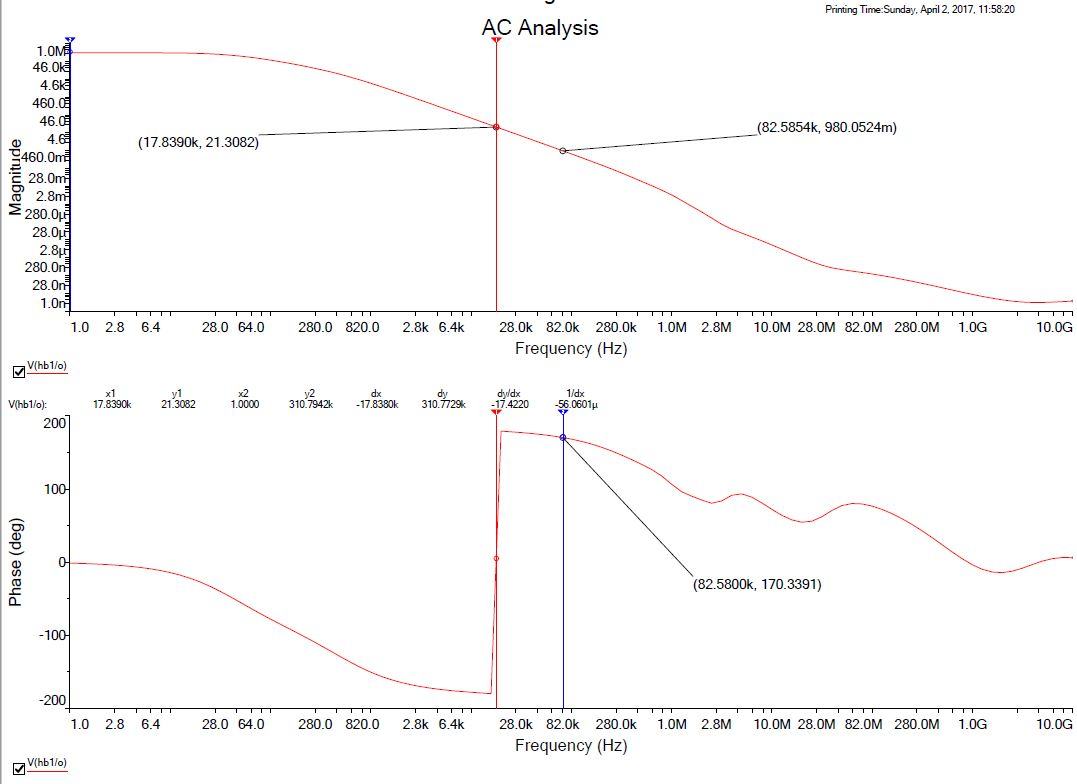
\includegraphics[width=\textwidth]{ffail.jpg}
\caption{集成运放bode图}
\label{bode}
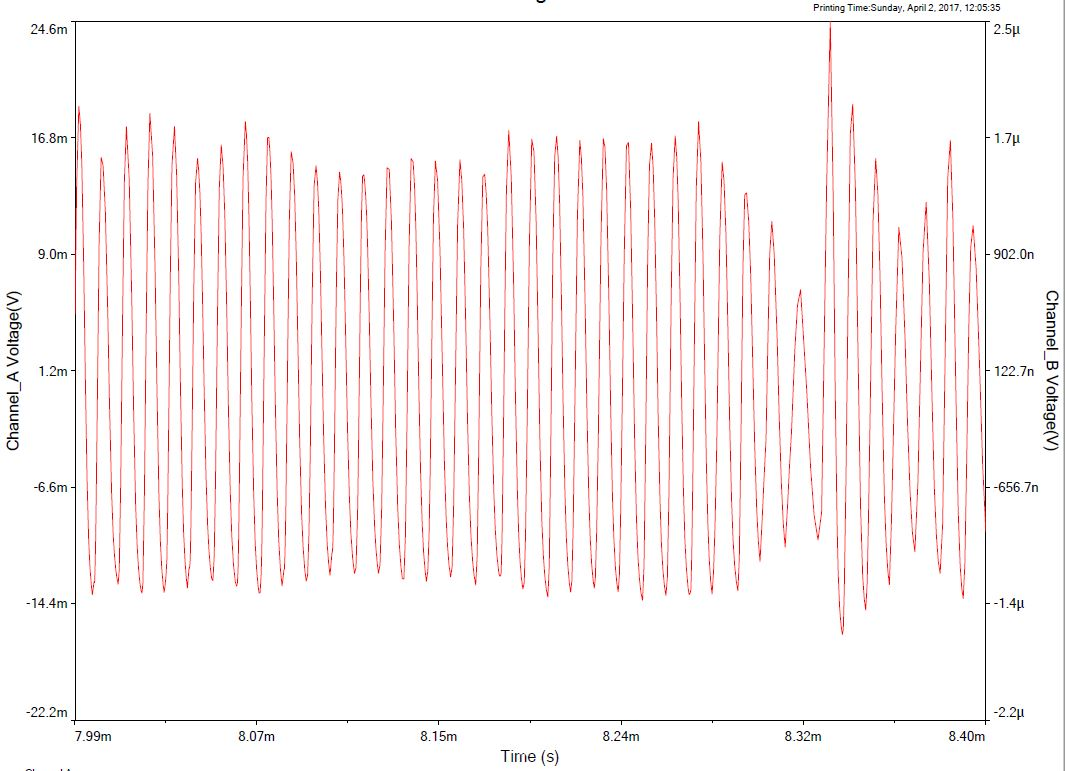
\includegraphics[width=\textwidth]{self.jpg}
\caption{自激震荡}
\label{exp}
\end{figure}
\subsection{自激震荡的消去}
在输出上级联超前补偿,经过调整可以消去自激震荡到nV量级一下,已经和噪声基本相同了,如图\ref{slu}所示发现失真得到明显的消去
\begin{figure}
\centering
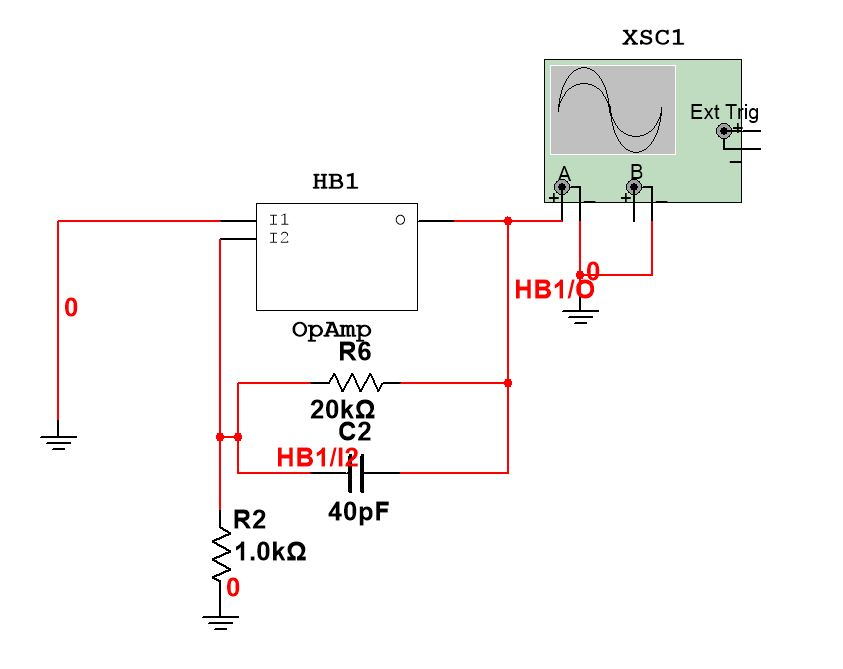
\includegraphics[width=\textwidth]{ok.jpg}
\caption{超前相位补偿}
\label{slu}
\end{figure}
\end{document}